%Generazione delle variabili che andranno a sostituire quelle del template `HomePage.tex`
\newcommand{\documento}{\PdP}
\newcommand{\nomedocumentofisico}{PianoDiProgetto.pdf}
\newcommand{\redazione}{\GR\\ & \GN}
\newcommand{\verifica}{\SM}
\newcommand{\approvazione}{\GR}
\newcommand{\uso}{Esterno}
\newcommand{\destinateTo}{\TV, \\ & \RC, \\ & \ZU}
\newcommand{\datacreazione}{05 Dicembre 2015}
\newcommand{\datamodifica}{11 Dicembre 2015}
\newcommand{\stato}{Sviluppo}

\def\TABELLE{false}	%abilita - disabilita l'indice delle tabelle
\def\FIGURE{false} 	%abilita - disabilita l'indice delle figure

%Layout del documento 
\documentclass[a4paper,11pt]{article}

%***IMPORTAZIONE PACKAGE***
\usepackage{ifthen}
\usepackage[italian]{babel}
\usepackage[utf8]{inputenc}
\usepackage[T1]{fontenc}
\usepackage{float}
\usepackage{chapterbib}
\usepackage{graphicx}
\usepackage[a4paper,top=2.5cm,bottom=2.5cm,left=2.5cm,right=2.5cm]{geometry}
\usepackage[colorlinks=true, urlcolor=black, citecolor=black, linkcolor=black]{hyperref}
\usepackage{booktabs}
\usepackage{fancyhdr}
\usepackage{totpages}
\usepackage{tabularx, array}
\usepackage{dcolumn}
\usepackage{epstopdf}
\usepackage{booktabs}
\usepackage{fancyhdr}
\usepackage{longtable}
\usepackage{calc}
\usepackage{datatool}
\usepackage[bottom]{footmisc}
\usepackage{listings} 
\usepackage{textcomp}
\usepackage{titlesec}
\usepackage{rotating} 
\usepackage{multirow}
\usepackage{placeins}
\usepackage{color}
\usepackage[table,usenames,dvipsnames]{xcolor}
\usepackage{hyperref}
\usepackage{makecell}
\usepackage{hyperref}


%***STILE PAGINA***
\pagestyle{fancy}
%no indentazione paragrafo
\setlength{\parindent}{0pt}

%***INTESTAZIONE***
\lhead{\Large{\progetto} \\ \footnotesize{\documento}}
\rhead{
\includegraphics[keepaspectratio = true, width = 25px] {../../Template/icone/LogoGruppo.png}}
\renewcommand{\headrulewidth}{0.4pt}  %Linea sotto l'intestazione

%***PIÈ DI PAGINA***
\lfoot{\textit{\gruppoLink}\\ \footnotesize{\email}}
\rfoot{\thepage} %per le prime pagine: mostra solo il numero romano
\cfoot{}
\renewcommand{\footrulewidth}{0.4pt}   %Linea sopra il piè di pagina

%***INSERIMENTO DI NUOVE SOTTOSEZIONI
\setcounter{secnumdepth}{7}		% mostra nel documento fino al livello 8 (1.2.3.4.5.6.7.8)
\setcounter{tocdepth}{7}			% mostra nell'indice fino al livello 8 (1.2.3.4.5.6.7.8)

%***LA SOTTOSEZIONE PARAGRAPH VIENE VISUALIZZATA COME UNA SECTION
\titleformat{\paragraph}{\normalfont\normalsize\bfseries}{\theparagraph}{1em}{}
\titlespacing*{\paragraph}{0pt}{3.25ex plus 1ex minus .2ex}{1.5ex plus .2ex}

\titleformat{\subparagraph}{\normalfont\normalsize\bfseries}{\thesubparagraph}{1em}{}
\titlespacing*{\subparagraph}{0pt}{3.25ex plus 1ex minus .2ex}{1.5ex plus .2ex}

\makeatletter
\newcounter{subsubparagraph}[subparagraph]
\renewcommand\thesubsubparagraph{%
  \thesubparagraph.\@arabic\c@subsubparagraph}
\newcommand\subsubparagraph{%
  \@startsection{subsubparagraph}    % counter
    {6}                              % level
    {\parindent}                     % indent
    {3.25ex \@plus 1ex \@minus .2ex} % beforeskip
    {0.75em}                           % afterskip
    {\normalfont\normalsize\bfseries}}
\newcommand\l@subsubparagraph{\@dottedtocline{6}{10em}{5.5em}} %gestione dell'indice
\newcommand{\subsubparagraphmark}[1]{}
\makeatother

\makeatletter
\newcounter{subsubsubparagraph}[subsubparagraph]
\renewcommand\thesubsubsubparagraph{%
  \thesubsubparagraph.\@arabic\c@subsubsubparagraph}
\newcommand\subsubsubparagraph{%
  \@startsection{subsubsubparagraph}    % counter
    {7}                              % level
    {\parindent}                     % indent
    {3.25ex \@plus 1ex \@minus .2ex} % beforeskip
    {0.75em}                           % afterskip
    {\normalfont\normalsize\bfseries}}
\newcommand\l@subsubsubparagraph{\@dottedtocline{7}{10em}{6.5em}} %gestione dell'indice
\newcommand{\subsubsubparagraphmark}[1]{}
\makeatother
\newcommand{\modificheuno} 
{	
	0.0.3 & Inseriti i primi riferimenti informativi & \specialcell[t]{\GN \\ \prog} & 2016-02-26
	\\\midrule
	0.0.2 & Stesura scopo del documento, scopo del prodotto , riferimenti normativi & \specialcell[t]{\GN \\ \prog} & 2016-02-26
	\\\midrule
	0.0.1 & Creato template documento & \specialcell[t]{\GN \\ \prog} & 2016-02-26
	\\\midrule
}
\newcommand{\modifichedue}
{
}

%Comandi generali
%Generali
\newcommand{\progetto}{QuizziPedia}
\newcommand{\gruppo}{TheFellowshipOfTheCode}
\newcommand{\gruppoLink}{\href{http://thefellowshipofthecode.github.io/}{TheFellowshipOfTheCode}}
\newcommand{\email}{\href{mailto:thefellowshipofthecode@gmail.com}{thefellowshipofthecode@gmail.com}}

%Documenti
\newcommand{\AdR}{Analisi dei Requisiti}
\newcommand{\NdP}{Norme di Progetto}
\newcommand{\PdP}{Piano di Progetto}
\newcommand{\SdF}{Studio di Fattibilità}
\newcommand{\PdQ}{Piano di Qualifica}
\newcommand{\VI}{Verbale Interno}
\newcommand{\VE}{Verbale Esterno}
\newcommand{\ST}{Specifica Tecnica}
\newcommand{\DDP}{Definizione di Prodotto}
\newcommand{\MU}{Manuale Utente}
\newcommand{\G}{Glossario}
\newcommand{\LdP}{Lettera di Presentazione}
\newcommand{\NdPv}{NormeDiProgetto\_v\_1\_0\_0}
\newcommand{\PdPv}{PianoDiProgetto\_v\_1\_0\_0}
\newcommand{\PdQv}{PianoDiQualifica\_v\_1\_0\_0}
\newcommand{\SdFv}{StudioDiFattibilità\_v\_1\_0\_0}

%Componenti del gruppo
\newcommand{\AF}{Alberto Ferrara}
\newcommand{\SM}{Simone Magagna}
\newcommand{\FB}{Franco Berton}
\newcommand{\MP}{Marco Prelaz}
\newcommand{\MV}{Mattia Varotto}
\newcommand{\GN}{Matteo Gnoato}
\newcommand{\GR}{Matteo Granzotto}

%Ruoli
\newcommand{\RdP}{Responsabile di Progetto}
\newcommand{\Res}{Responsabile}
\newcommand{\Amm}{Amministratore}
\newcommand{\Ver}{Verificatore}
\newcommand{\Prog}{Progettista}
\newcommand{\Progr}{Programmatore}
\newcommand{\Ana}{Analista}
\newcommand{\RdPs}{Responsabili di Progetto}
\newcommand{\Ress}{Responsabile}
\newcommand{\Amms}{Amministratori}
\newcommand{\Vers}{Verificatori}
\newcommand{\Progs}{Progettisti}
\newcommand{\Progrs}{Programmatori}
\newcommand{\Anas}{Analisti}

%Professori e proponente
\newcommand{\TV}{Prof. Tullio Vardanega}
\newcommand{\RC}{Prof. Riccardo Cardin}
\newcommand{\ZU}{Zucchetti S.P.A.}
\newcommand{\proponente}{Zucchetti S.P.A.}

\newcommand{\diaryEntry}[5]{#2 & \emph{#4} & #3 & #5 & #1\\ \hline}

%comando per una nuova riga nella tabella del diario delle modifiche
\newcommand{\specialcell}[2][c]{%
	\begin{tabular}[#1]{@{}c@{}}#2\end{tabular}}

\renewcommand*\sectionmark[1]{\markboth{#1}{}}
\renewcommand*\subsectionmark[1]{\markright{#1}}

%Pediodi di lavoro 
\newcommand{\AR}{Analisi dei Requisiti}
\newcommand{\AD}{Analisi dei Requisiti in Dettaglio}
\newcommand{\PA}{Progettazione Architetturale}
\newcommand{\PD}{Progettazione di Dettaglio}
\newcommand{\CO}{Codifica}
\newcommand{\VV}{Verifica e Validazione}

% Revisioni
\newcommand{\RR}{Revisione dei Requisiti}
\newcommand{\RP}{Revisione di Progettazione}
\newcommand{\RQ}{Revisione di Qualifica}
\newcommand{\RA}{Revisione di Accettazione}

% Comandi analisi dei requisiti
\newcommand{\uau}{utente autenticato}
\newcommand{\uaus}{utenti autenticati}
\newcommand{\uaupro}{utente autenticato pro}
\newcommand{\uauspro}{utenti autenticati pro}

\newcommand{\myincludegraphics}[2][]{%
	\setbox0=\hbox{\phantom{X}}%
	\vtop{
		\hbox{\phantom{X}}
		\vskip-\ht0
		\hbox{\includegraphics[#1]{#2}}}}

\begin{document}
	
%inclusione template HomePage
\begin{center}

%
\includegraphics[width=1em]{../../../Template/icone/LogoGruppo.png}
\begin{large} \textbf{\gruppoLink} \end{large}
%
\includegraphics[width=1em]{../../../Template/icone/LogoGruppo.png}
\vspace{0.2em}

\hrule
\vspace{3em}


\includegraphics[keepaspectratio = true, width=8cm]{../../../Template/icone/LogoGruppo.png}

%Prima pagina senza intestazione né piè di pagina	
\thispagestyle{empty}

%Le informazioni del documento sono ancorate a fine pagina
\vfill

%Copertina
\begin{center} 
  \begin{Huge}
  {\fontsize{15mm}{20mm}\selectfont \progetto} 
  \end{Huge}
\end{center}

\begin{Huge} \documento \end{Huge}

\begin{center}
\textbf{Informazioni sul documento} \\ \vspace{2em}
\small
\begin{tabular}{r|l}
	\textbf{Nome Documento} & \nomedocumentofisico \\
	\textbf{Versione}	& 1\\
	\textbf{Data di Creazione} & \datacreazione\\
	\textbf{Data ultima modifica} & \datamodifica\\
	\textbf{Stato} & \stato \\
	\textbf{Redazione}	& \redazione\\
	\textbf{Verifica}	& \verifica\\
	\textbf{Approvazione}	& \approvazione\\
	\textbf{Uso}  & \uso\\
	\textbf{Distribuzione} & \gruppo \\
	\textbf{Destinato a}  &  \destinateTo \\
	\textbf{Email di riferimento} & \email
\end{tabular}
\end{center}

\normalsize
%Sommario
\textbf{Sommario\\} 
Documento contenente le norme di progetto che il gruppo \textit{\gruppo} seguirà durante tutte le fasi di realizzazione del prodotto \textit{\progetto}.

%\vfill %cosa fa?
\end{center}
\clearpage


%Registro delle modifiche e indice 
%si usa la numerazione romana per gli indici e la tabella delle modifiche
\pagenumbering{Roman}
\newpage
%***REGISTRO DELLE MODIFICHE***
%Vari comandi per la struttura della tabella, NON MODIFICARE!
\begin{center}
	\Large{\textbf{Registro delle modifiche}}
	\\\vspace{0.5cm}
	\normalsize
	\begin{tabularx}{\textwidth}{cXcc}
		\textbf{Versione} & \textbf{Descrizione} & \textbf{Autore e Ruolo} & \textbf{Data} \\\toprule
		\modifiche
		\bottomrule
\end{tabularx}
\end{center}
\newpage
%Inserisce il link all'indice
%\addcontentsline{toc}{section}{Indice}
\tableofcontents
\clearpage 

%Se è stata impostata a true la variabile per la lista delle tabelle, la mostra
\ifthenelse{\equal{\TABELLE}{true}} 
{\listoftables \newpage}{}

%Se è stata impostata a true la variabile per la lista delle figure, la mostra
\ifthenelse{\equal{\FIGURE}{true}}
{\listoffigures \newpage}{}

%Da qui comincia la numerazione normale
\pagenumbering{arabic}

%Imposta il formato di visualizzazione
\rfoot{\thepage~di~\pageref{TotPages}}

%sezioni documento
\newpage
\section{Introduzione}

\subsection{Scopo del documento}
Il presente documento ha lo scopo di definire in dettaglio la struttura e il funzionamento delle componenti del progetto \progetto. Questo documento servirà come guida per i \textit{\Progrs} del gruppo \gruppo fornendo direttive e vincoli per la realizzazione del \textit{progetto\ped{G}}.

\subsection{Scopo del prodotto}
Lo scopo del prodotto è di permettere la creazione e gestione di questionari in grado di identificare le lacune dei candidati prima, durante e al termine di un corso di formazione. 
\\Il sistema dovrà offrire le seguenti funzionalità:
\begin{itemize}
	\item
	Archiviare questionari in un server suddivisi per argomento;
	\item
	Somministrare all'utente, tramite un'interfaccia, questionari specifici per argomento scelto;
	\item
	Verificare e valutare i questionari scelti dagli utenti in base alle risposte date.
\end{itemize}
La parte destinata ai creatori di questionari dovrà essere fruibile attraverso un \textit{browser\ped{G}} desktop, abilitato all'utilizzo delle tecnologie \textit{HTML5\ped{G}}, \textit{CSS3\ped{G}} e \textit{JavaScript\ped{G}}. La parte destinata agli esaminandi sarà utilizzabile su qualunque dispositivo: dal personal computer ai tablet e smartphone.

\subsection{Glossario}
Al fine di evitare ogni ambiguità i termini tecnici del dominio del progetto, gli acronimi e le parole che necessitano di ulteriori spiegazioni saranno nei vari documenti marcate con il pedice \ped{G} e quindi presenti nel documento \textit{\G}.


\subsection{Riferimenti}
\subsubsection{Normativi}
\begin{itemize}
	\item \textit{\NdPv};
	\item \textit{\AdRvDue};
\end{itemize}
\subsubsection{Informativi}
\begin{itemize}
	\item \textbf{Ingegneria del software - Ian Sommerville - 8a edizione (2007)}: \\
	Parte terza: Progettazione, capitolo 11: Progettazione architetturale, Capitolo 14: Progettazione orientata agli oggetti;
	\item \textbf{Design Patterns} - Erich Gamma, Richard Helm, Ralph Johnson, John Vlissides - 1a edizione italiana (2006);
	\item \textbf{Slide dell'insegnamento - Design patterns:}
	\begin{itemize}
		\item Strutturali: \url{http://www.math.unipd.it/~tullio/IS-1/2015/Dispense/E07.pdf};
		\item Creazionali: \url{http://www.math.unipd.it/~tullio/IS-1/2015/Dispense/E08.pdf}
		\item Comportamentali: \url{http://www.math.unipd.it/~tullio/IS-1/2015/Dispense/E09.pdf}
		\item Architetturali:
			\begin{itemize}
				\item \url{http://www.math.unipd.it/~rcardin/sweb/Design%20Pattern%20Architetturali%20-%20Model%20View%20Controller_4x4.pdf};
				\item \url{http://www.math.unipd.it/~rcardin/sweb/Design%20Pattern%20Architetturali%20-%20Dependency%20Injection_4x4.pdf}.
			\end{itemize} 
	\end{itemize}
	\item \textbf{Martin Fowler - UML\ped{G} Distilled} - 2nd edition;
	\item \textbf{Slide dell'insegnamento - Diagrammi delle classi}: \\
		\url{http://www.math.unipd.it/~tullio/IS-1/2015/Dispense/E03.pdf}
	\item \textbf{Slide dell'insegnamento - Diagrammi dei packages:} \\
		\url{http://www.math.unipd.it/~tullio/IS-1/2015/Dispense/E04.pdf}
	\item \textbf{Slide dell'insegnamento - Diagrammi di sequenza:} \\
		\url{http://www.math.unipd.it/~tullio/IS-1/2015/Dispense/E05.pdf}
	\item \textbf{Documentazione del \textit{Framework\ped{G}MEAN\ped{G}.js}:} \\
		\url{http://learn.mean.io/}
	\item \textbf{Documentazione della \textit{piattaforma} Node.js:} \\
		\url{https://nodejs.org/api/}
	\item \textbf{Giuda all'utilizzo dei middleware Express:} \\
		\url{http://expressjs.com/it/guide/using-middleware.html}
	\item \textbf{Guida all'utilizzo dei middleware Passport:} \\
		\url{http://passportjs.org/docs}
	\item \textbf{Manuale del database \textit{MongoDB\ped{G}}:} \\
		\url{https://docs.mongodb.org/manual/}
	\item \textbf{Documentazione dell'interfaccia REST:}
		\begin{itemize}
			\item \textit{Descrizione di REST:} \url{https://it.wikipedia.org/wiki/Representational_State_Transfer}
			\item \textit{Descrizione risorse REST:} \url{http://stashboard.readthedocs.org/en/latest/restapi.html}
		\end{itemize}
	\item \textbf{Documentazione del \textit{framework\ped{G} AngularJS\ped{G}}:} \\
		\begin{itemize}
			\item \textit{Documentazione generica:} \url{https://docs.angularjs.org/guide}
			\item \textit{Documentazione servizio \$http:} \url{https://docs.angularjs.org/api/ng/service/\$http}
			\item \textit{Documentazione servizio \$location:} \url{https://docs.angularjs.org/api/ng/service/\$location}
			\item \textit{Documentazione servizio \$windows:} \url{https://docs.angularjs.org/api/ng/service/\$window}
			\item \textit{Documentazione servizio \$ruoteParams:} \url{https://docs.angularjs.org/api/ngRoute/service/\$routeParams}
			\item \textit{Documentazione servizio \$q:} \url{https://docs.angularjs.org/api/ng/service/\$q}
		\end{itemize}
	\item \textbf{Documentazione del \textit{framework\ped{G}} Material for Angular:} \\
		\url{https://material.angularjs.org/latest/}
	\item \textbf{Documentazione del \textit{framework\ped{G}} Chart.js} \\
		\url{http://www.chartjs.org/docs/}
	\item \textbf{Documentazione del \textit{wrapper\ped{G}} Angles.js} \\
		\url{https://github.com/gonewandering/angles}
	\item \textbf{Documentazione del \textit{framework\ped{G}} TextAngular.js} \\
		\url{https://github.com/fraywing/textAngular/wiki/textAngular-Docs-v1.1.x}
	\item \textbf{Guida all'utilizzo della direttiva \textit{ng-file-upload}} \\
		\url{https://github.com/danialfarid/ng-file-upload}
	\item \textbf{Documentazione di \textit{jison\ped{G}} per la definizione della grammatica di QML} \\
		\url{http://zaa.ch/jison/docs/}
\end{itemize} 
\newpage
\section{Pianificazione}
Per migliorare lo sviluppo del progetto, il \textit{team\ped{G}} ha deciso di suddividere il carico di lavoro in sei periodi:
\begin{itemize}
	\item \textbf{\AR (AR)};
	\item \textbf{\AD (AD)};
	\item \textbf{\PA (PA)};
	\item \textbf{\PD (PD)};
	\item \textbf{\CO (CO)};
	\item \textbf{\VV (VV)}.
\end{itemize}

Per evidenziare le attività principali di un periodo, ad ognuno di essi viene associato un \textit{diagramma di Gantt\ped{G}}. 
Ogni attività, a propria volta, può essere suddivisa in sotto-attività e fare riferimento ad una o più risorse.
Una \textit{milestone\ped{G}} può essere esterna, coincidendo con le date di consegna dei documenti, o interna, ovvero un punto di revisione stabilito dal \textit{team\ped{G}}. 
All'interno di un \textit{diagramma di Gantt\ped{G}} vengono rappresentate con dei rombi neri. 
Il momento in cui un periodo termina coincide sempre con una \textit{milestone\ped{G}}.\\ 
La rappresentazione temporale delle attività nel \textit{diagramma di Gantt\ped{G}} avviene mediante linee nere, le cui estremità sono delle frecce rivolte verso il basso. 
I \textit{diagrammi di Gantt\ped{G}} permettono inoltre, grazie all'uso di frecce, di rappresentare le dipendenze tra attività e sotto-attività.
La conseguenza di un ritardo su un'attività è lo slittamento temporale di tutte le attività ad essa correlate. \\

Nei \textit{diagrammi di Gantt\ped{G}} le sotto-attività sono suddivise nel modo seguente:
\begin{itemize}
	\item \textbf{Critiche}: lo svolgimento di queste attività è necessario per la riuscita del progetto nei tempi prestabiliti. Un ritardo sarebbe di grave danno per l'efficienza del \textit{team\ped{G}} in ottica del raggiungimento della \textit{Milestone\ped{G}}. \\ 
	Le attività di questo tipo vengono rappresentate all'interno del \textit{diagramma di Gantt\ped{G}} con il colore \textit{rosso}.
	\item \textbf{Non critiche}: queste attività possono essere svolte parallelamente alle sotto-attività critiche. Un ritardo in tali attività non comporta uno slittamento temporale di tutto il progetto.
	Le attività di questo tipo vengono rappresentate all'interno del \textit{diagramma di Gantt\ped{G}} con il colore \textit{blu}.
\end{itemize}
Si è deciso di non riportare i diagrammi \textit{PERT\ped{G}} in quanto poco leggibili data la moltitudine di nodi presenti; quindi si è scelto di presentare i soli \textit{diagrammi di Gantt\ped{G}} riportando anche le risorse impegnate per ciascuna attività.

\subsection{Suddivisione delle attività}

\subsubsection{\AR}
\textbf{Periodo:} dal 2015-12-08 al 2016-01-22.\\
Questo periodo inizia in concomitanza alla formazione del gruppo e termina con la consegna dei documenti per la \textbf{\RR}.\\ 
Questo periodo prevede di stilare i seguenti documenti:
\begin{itemize}
		\item \textit{\NdP}: questo è il primo documento redatto in ordine cronologico poiché norma tutto l'operato del \textit{team\ped{G}} riguardo la stesura dei documenti, delle comunicazioni, etc. ed è indipendente dal capitolato scelto. E' l’\textit{Amministratore di Progetto} a redigere questo documento inserendovi le norme che il \textit{team\ped{G}} dovrà seguire durante lo svolgimento di tutte le attività. I \textit{\Vers} certificheranno che tutte le norme siano state effettivamente osservate durante le diverse attività;
		\item \textit{\SdF}: in questo documento vengono analizzati tutti i capitolati proposti. Per ognuno viene analizzato il dominio tecnologico e applicativo valutandone i fattori positivi e negativi. Risulta essere un'attività	critica perché definisce il progetto sul quale il gruppo andrà a lavorare e blocca la stesura del documento di \textit{\AdR};
		\item \textit{\AdR}: redatto dagli \textit{\Anas}, è l'analisi approfondita del capitolato scelto con lo \textit{\SdF};
		\item \textit{\PdP}: redatto dal \textit{\RdP}, individua tutte le attività necessarie allo svolgimento del progetto e le assegna alle risorse disponibili distribuendo il carico di lavoro in maniera uniforme.
		La priorità di questo documento è alta poiché vincola tutte attività svolte dal \textit{team\ped{G}};
		\item \textit{\PdQ}: steso dal \textit{\Ver}, definisce come devono essere effettuate le verifiche al fine di consegnare un prodotto di qualità;
		\item \textit{\G}: scritto in maniera incrementale dai redattori dei diversi documenti e contiene la spiegazione di alcuni termini utilizzati nei vari documenti, al fine di eliminare ogni possibile ambiguità di significato;
		\item \textit{\LdP}: documento che dichiara l’interesse del gruppo a partecipare alla gara d’appalto.
\end{itemize}
Ogni documento sopraccitato oltre che stilato verrà anche verificato; la verifica dei presenti documenti è considerata un'attività critica.
In questa fase i ruoli maggiormente interessati sono quelli di \textit{\Amm}, \textit{\Res}, \textit{\Ana} e \textit{\Ver}. 
\begin{sidewaysfigure}
	\centering
	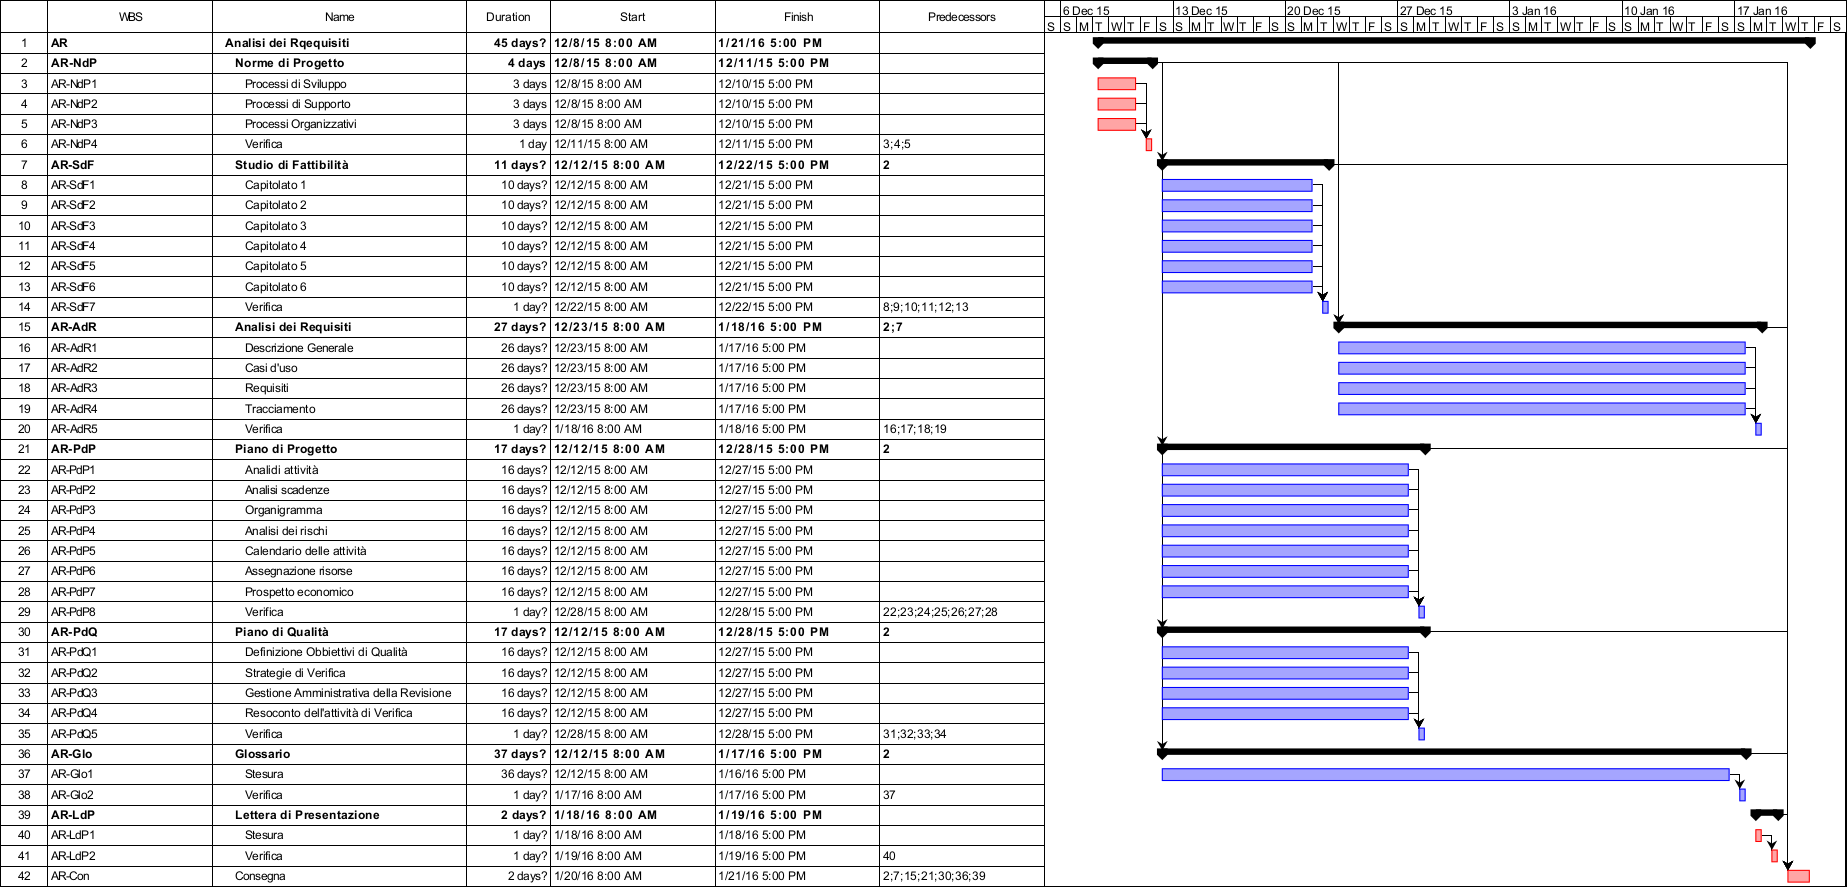
\includegraphics[keepaspectratio = true, width=23cm]{immagini/PdP_AnalisiDeiRequisitiGantt.png}
	\caption{\textit{Diagramma di Gantt\ped{G}} relativo al periodo di \AR.}\label{etichetta}
\end{sidewaysfigure}
\newpage

\subsubsection{\AD}
\textbf{Periodo:} dal 2016-01-23 al 2016-02-22. \\
Il periodo di \AD inizia subito dopo la consegna dei documenti per la \RR e termina con l'inizio del periodo successivo, quello della \PA. Il termine fissato corrisponde ad una \textit{milestone\ped{G}} interna. \\
In questo periodo il gruppo mira a consolidare ed ampliare i requisiti richiesti dal sistema e a migliorare il documento di \textit{\AdR} attuando le correzioni in base all'esito della \RR.
Vengono inoltre corretti e verificati anche gli altri documenti. 
In questa fase i ruoli maggiormente interessati sono quelli di \textit{\Ana} e \textit{\Ver}.  
\begin{center}
	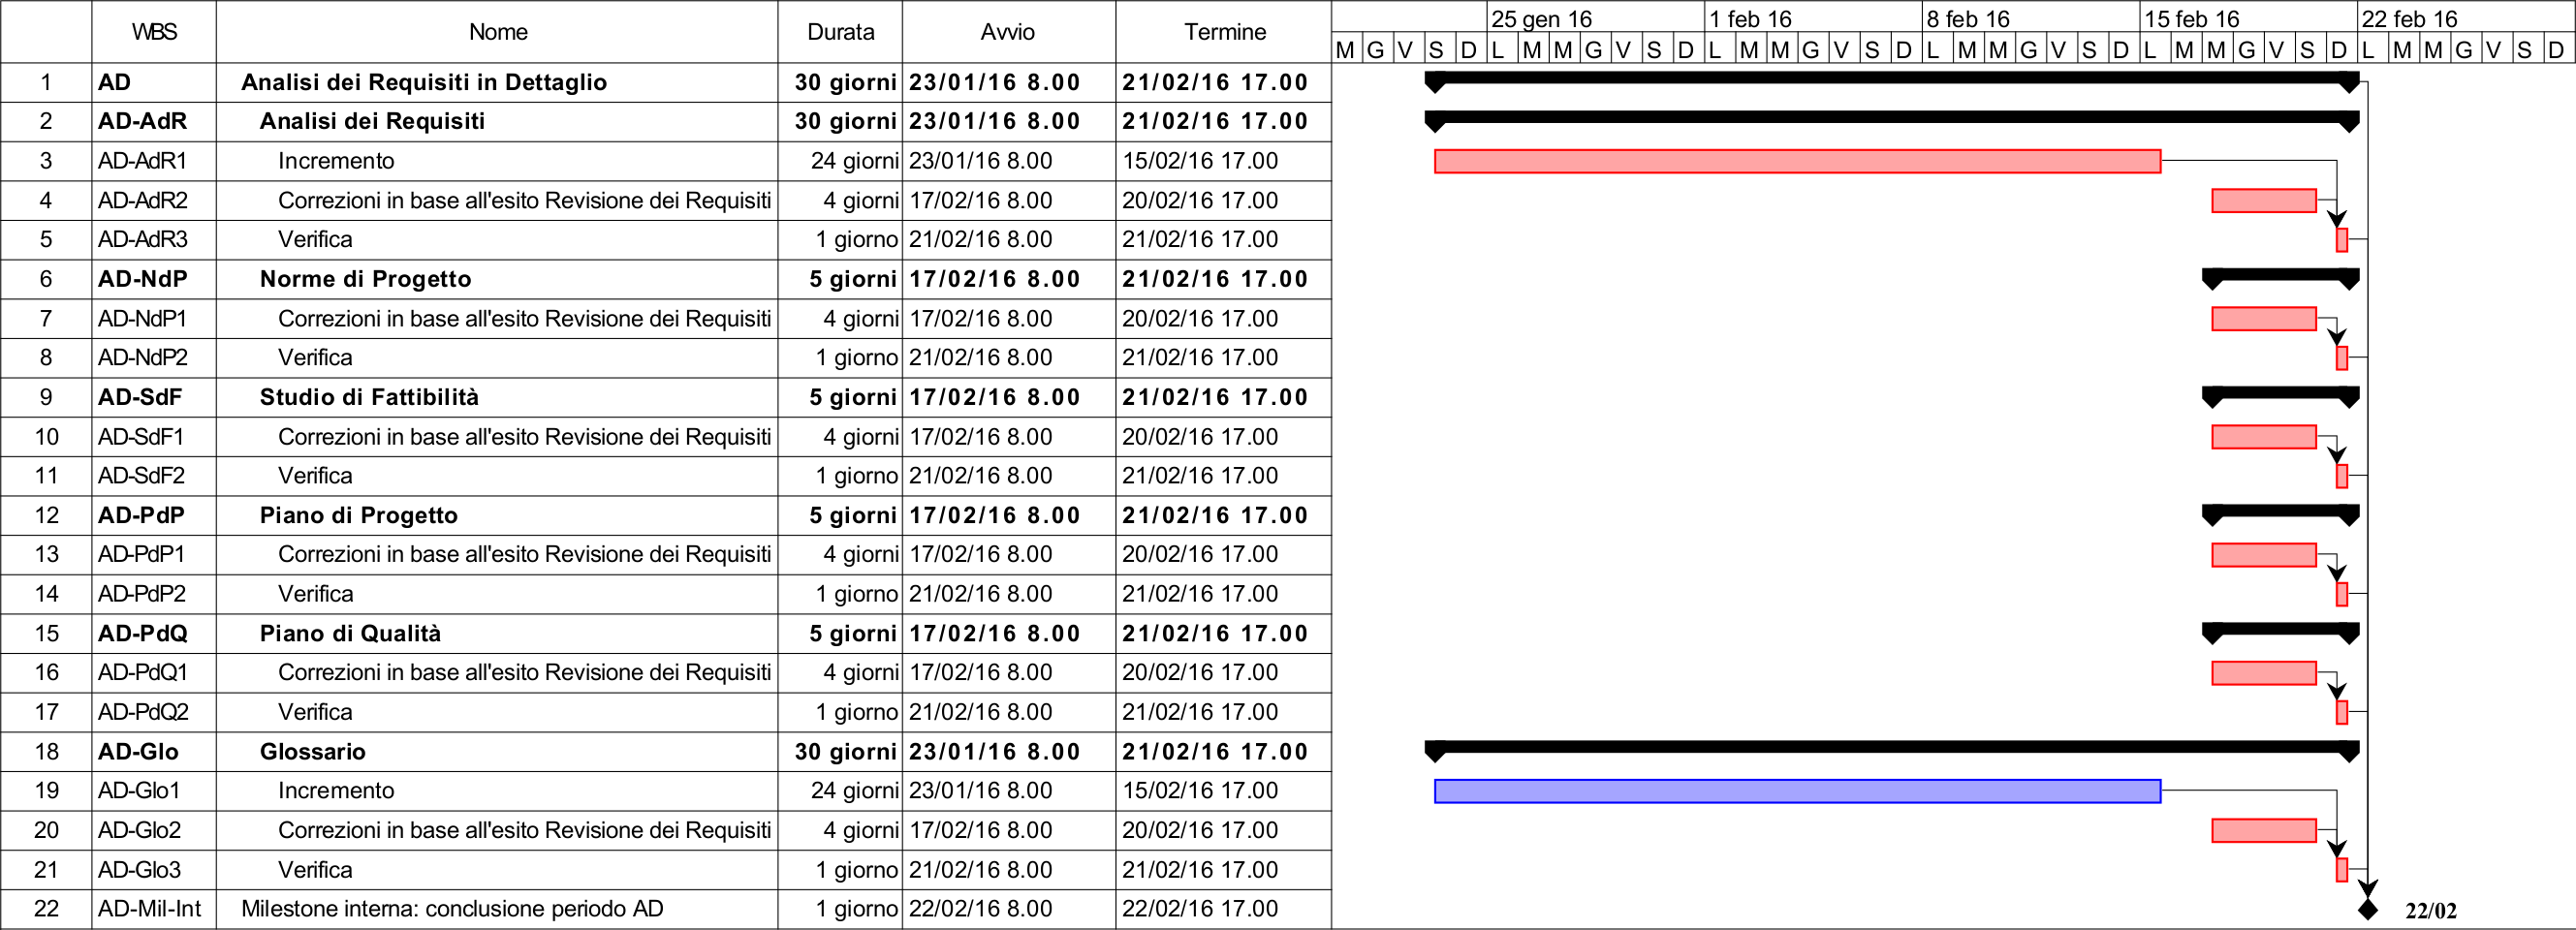
\includegraphics[keepaspectratio = true, width=16cm]{immagini/PdP_AnalisiDeiRequisitiInDettaglioGantt.png}
\end{center}
\begin{figure}[h]
	\caption{\textit{Diagramma di Gantt\ped{G}} relativo al periodo di \AD.}\label{etichetta}
\end{figure}

\subsubsection{\PA}
\textbf{Periodo:} dal 2016-02-23 al 2016-03-20. \\
Il periodo di \PA, inizia dopo quello di \AD e si conclude con una \textit{milestone\ped{G}} interna di \RdP minima. L'obbiettivo di questo periodo è la stesura della progettazione ad alto livello del sistema e prevede di svolgere le seguenti attività:
\begin{itemize}
	\item Redigere il documento di \textit{\ST}: il \textit{\Prog} deve descrivere le scelte progettuali di alto livello effettuate, i \textit{design pattern\ped{G}} scelti per la realizzazione del prodotto e l'architettura generale del software. Inoltre deve venir effettuato il tracciamento dei requisiti;  
	\item Incrementare i documenti di: \textit{\NdP},\textit{\PdP} e \textit{\PdQ};
	\item Verificare tutti i documenti sopraccitati.
\end{itemize}
In questa fase i ruoli maggiormente interessati sono quelli di \textit{\Amm}, \textit{\Res}, \textit{\Prog} e \textit{\Ver}. 
\begin{center}
	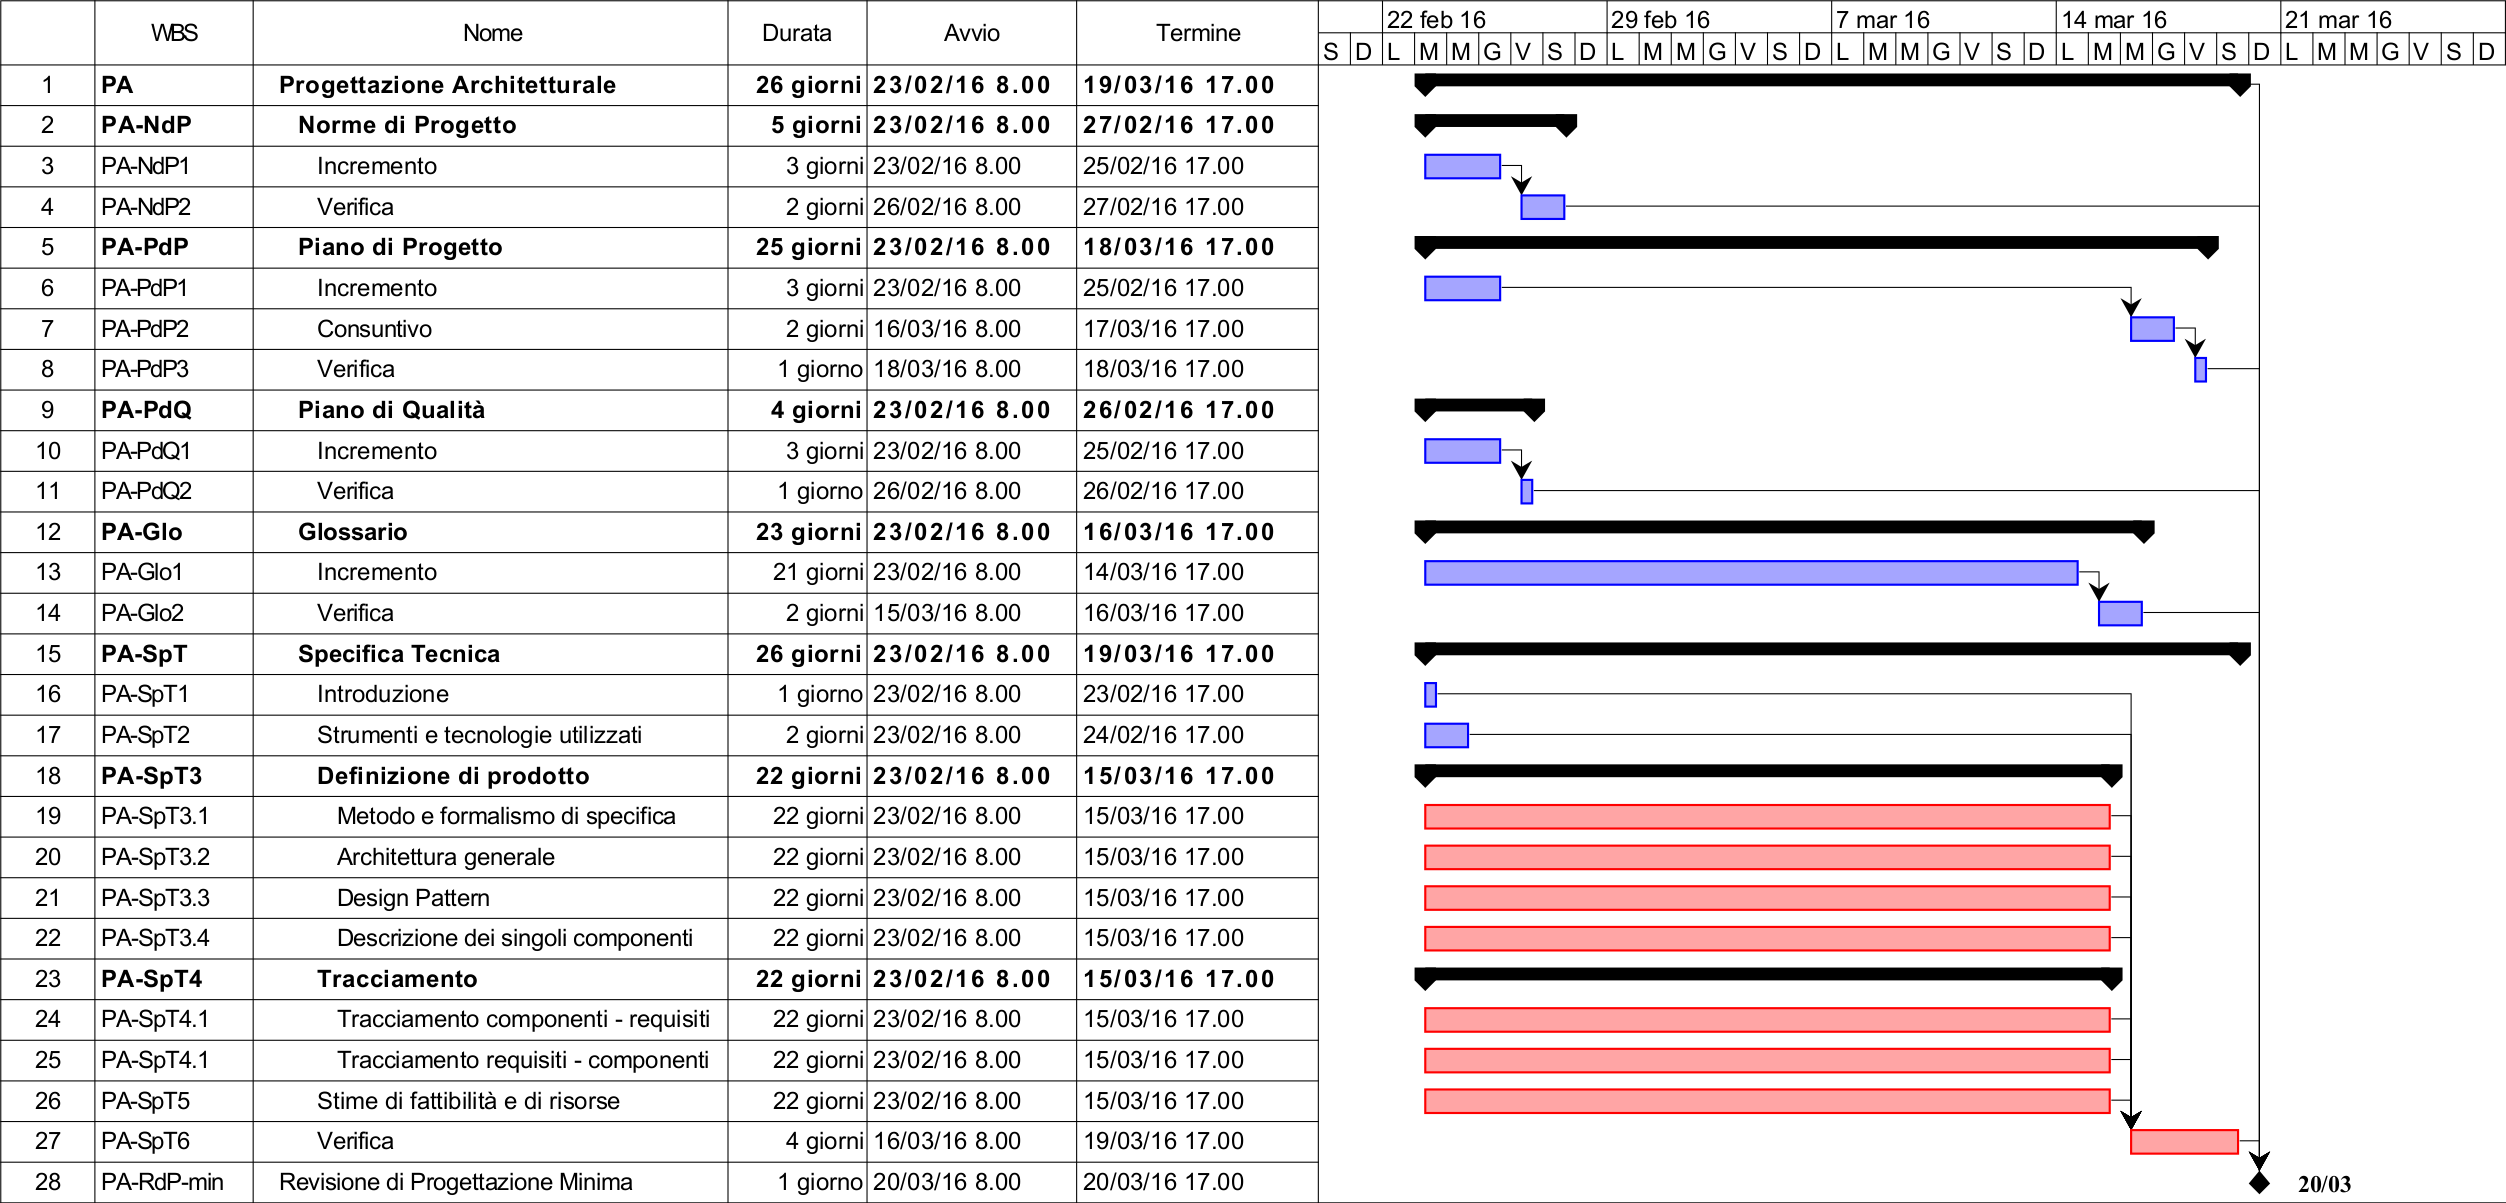
\includegraphics[keepaspectratio = true, width=16cm]{immagini/PdP_ProgettazioneArchitetturaleGantt.png}
\end{center}
\begin{figure}[h]
	\caption{\textit{Diagramma di Gantt\ped{G}} relativo al periodo di \PA.}\label{etichetta}
\end{figure}

\subsubsection{\PD}
\textbf{Periodo:} dal 2016-03-21 al 2016-04-11. \\
Il periodo di \PD, inizia dopo quello di \PA e si conclude con la consegna dei documenti per la \RP. L'obbiettivo di questo periodo è la stesura, in modo dettagliato, dell'intero sistema, specificando in modo approfondito il comportamento e l'iterazione tra i vari componenti. \\
Prevede di svolgere le seguenti attività:
\begin{itemize}
	\item Redigere il documento di \textit{\DDP}: il \textit{\Prog} deve descrivere il comportamento e le iterazioni tra i vari componenti del sistema basandosi sul documento di \textit{\ST};  
	\item Incrementare i documenti di: \textit{\NdP},\textit{\PdP}, \textit{\PdQ}, \textit{\ST} e \textit{\G};
	\item Verificare tutti i documenti sopraccitati.
\end{itemize}
In questa fase i ruoli maggiormente interessati sono quelli di \textit{\Amm}, \textit{\Res}, \textit{\Prog} e \textit{\Ver}. 
\begin{center}
	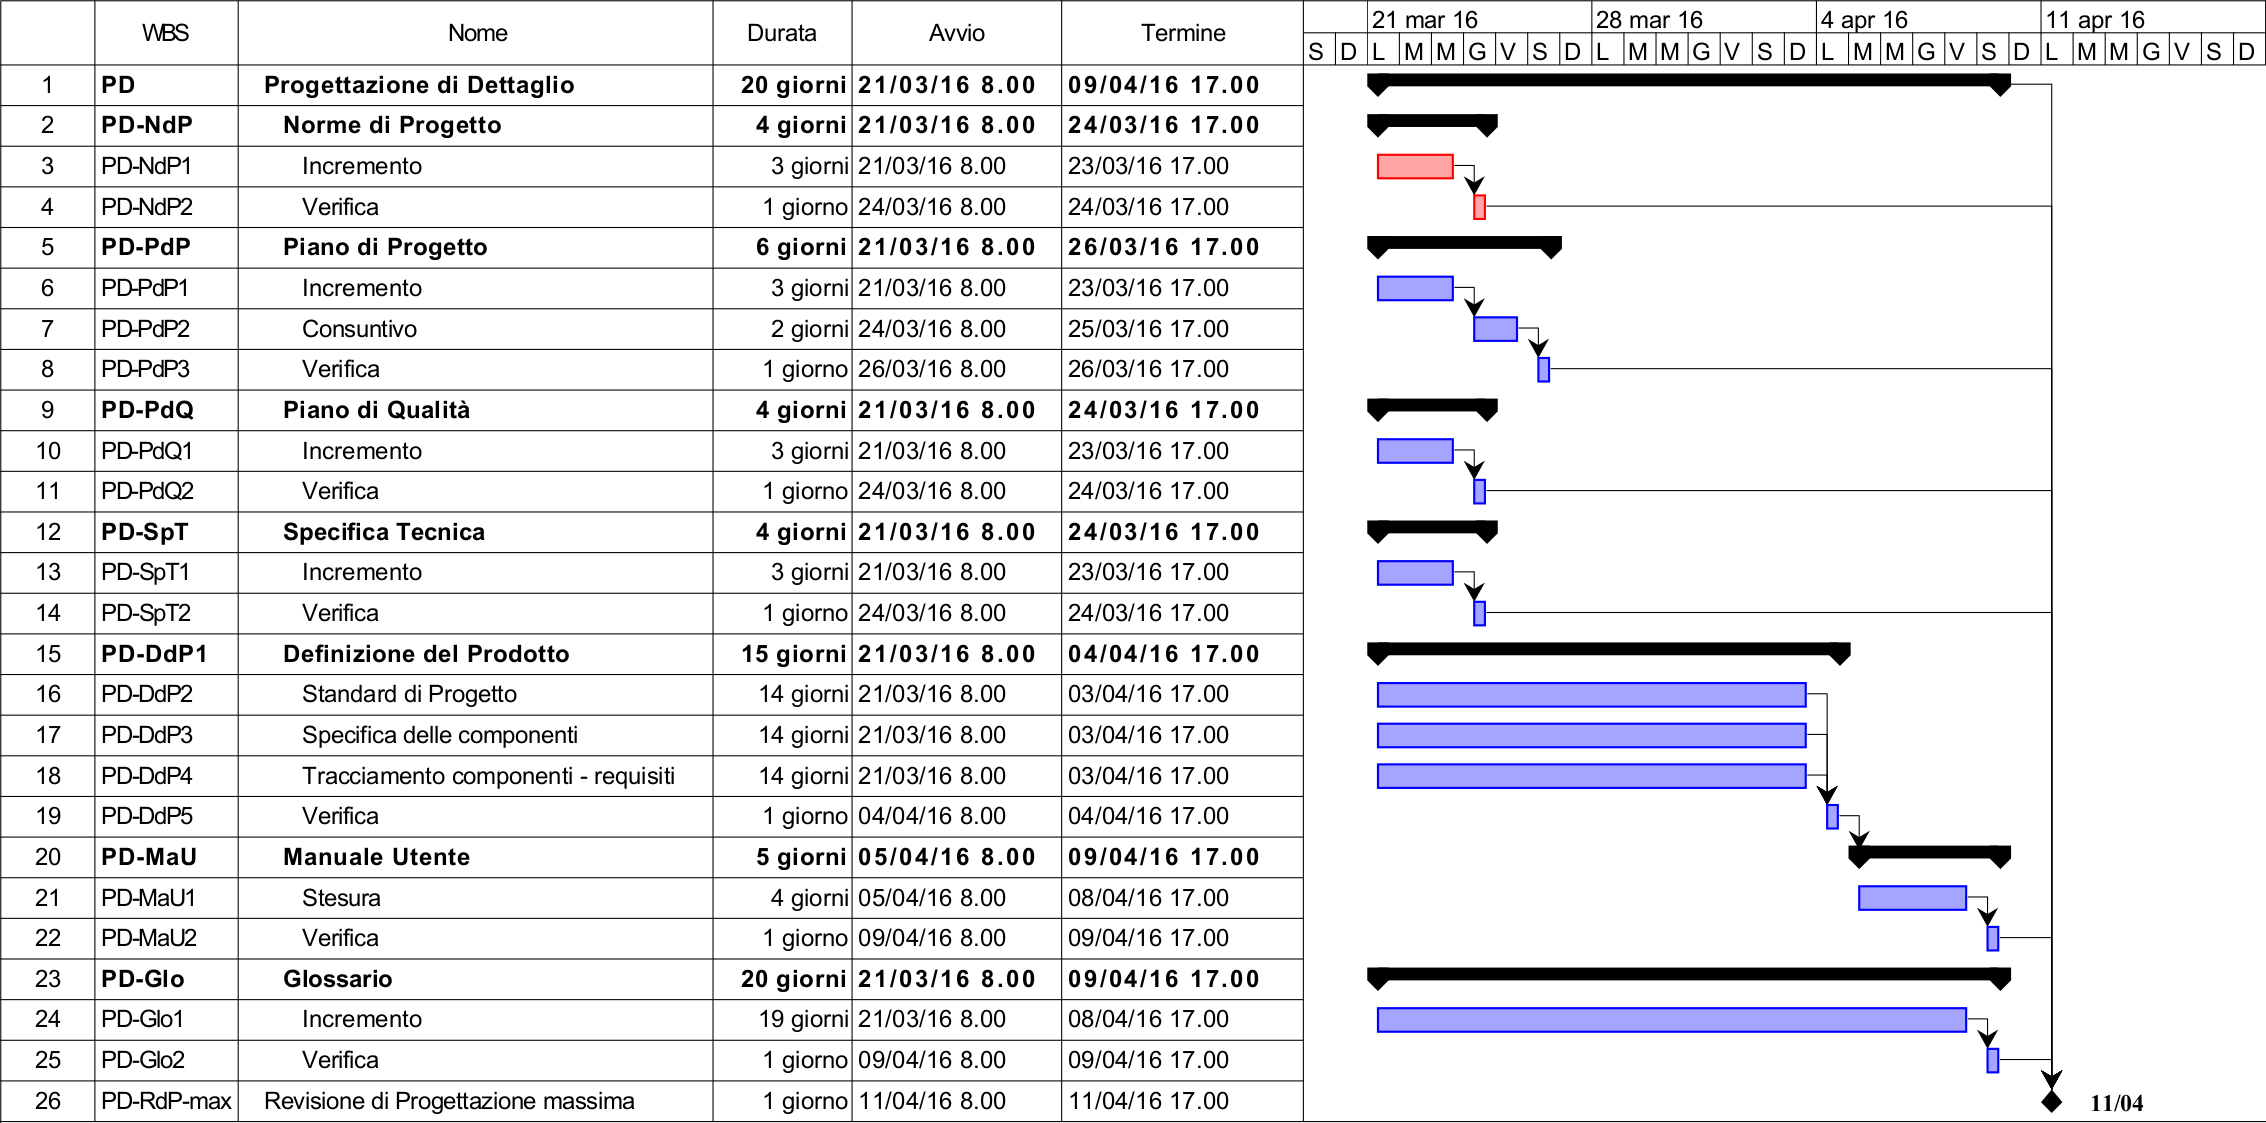
\includegraphics[keepaspectratio = true, width=16cm]{immagini/PdP_ProgettazioneDiDettaglioGantt.png}
\end{center}
\begin{figure}[h]
	\caption{\textit{Diagramma di Gantt\ped{G}} relativo al periodo di \PD.}\label{etichetta}
\end{figure}

\subsubsection{\CO}
\textbf{Periodo:} dal 2016-04-19 al 2016-05-16. \\
Il periodo di \CO, inizia dopo quello di \PD  e si conclude con la consegna del prodotto alla \RQ. L'obbiettivo in questo periodo è di consegnare un prodotto qualificato e prevede di svolgere le seguenti attività:
\begin{itemize}
	\item \textbf{\CO}: attenendosi a quanto scritto dai \textit{\Progs} nel documento di \textit{\DDP}, i \textit{\Progrs} dovranno sviluppare il codice del prodotto software.\\
	L'attività di \CO, dopo un primo momento, prevede due cicli incrementali per il miglioramento di parti del sistema esistenti o per l'aggiunta di funzionalità al sistema stesso. \\
	Ogni incremento prevede tre attività:
	\begin{itemize}
		\item Progettazione dell'incremento da parte dei \textit{\Progs};  
		\item Codifica da parte dei \textit{\Progrs} dell'incremento;
		\item Verifica dell'incremento. 
	\end{itemize}
	\item \textit{\MU}: documento destinato all'utilizzatore finale del prodotto che ne descrive le linee guida per il corretto utilizzo;
	\item Incrementare i documenti di: \textit{\NdP},\textit{\PdP}, \textit{\PdQ} e \textit{\G};
	\item Verificare tutti i documenti sopraccitati.
\end{itemize}
In questa fase i ruoli maggiormente interessati sono quelli di \textit{\Amm}, \textit{\Res}, \textit{\Prog}, \textit{\Progr} e \textit{\Ver}. 
\begin{center}
	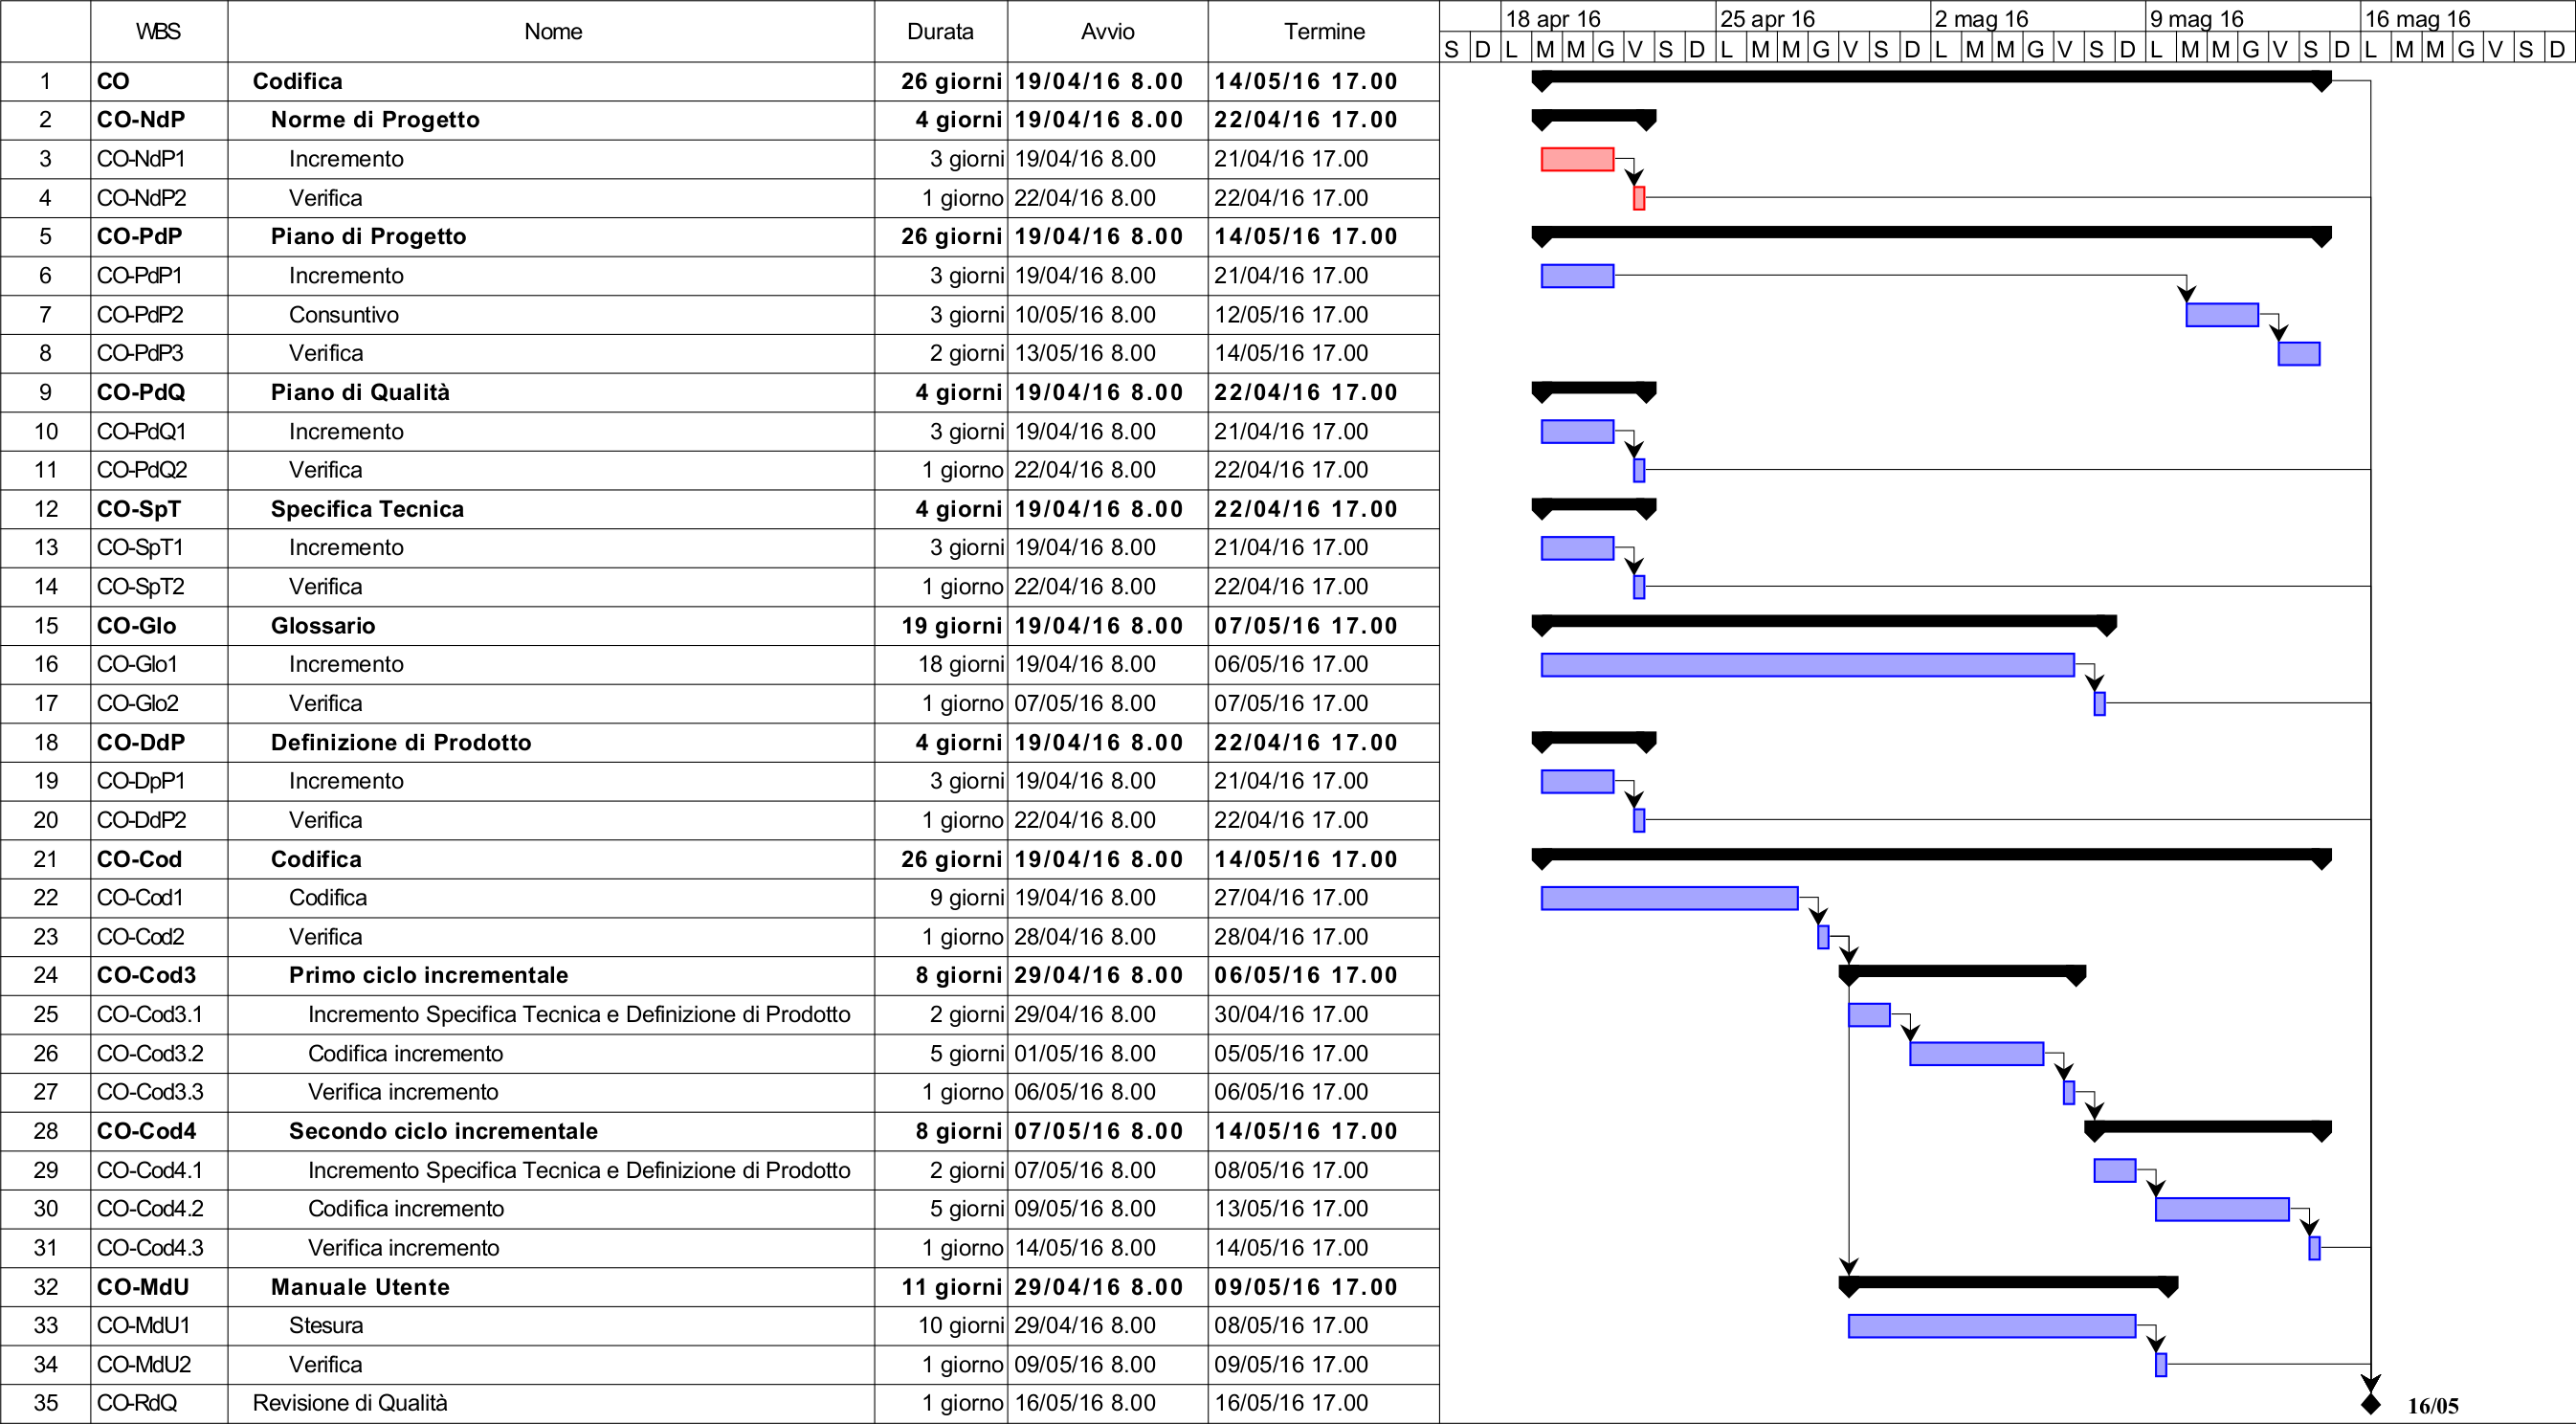
\includegraphics[keepaspectratio = true, width=16cm]{immagini/PdP_CodificaGantt.png}
\end{center}
\begin{figure}[h]
	\caption{\textit{Diagramma di Gantt\ped{G}} relativo al periodo di \CO.}\label{etichetta}
\end{figure}

\subsubsection{\VV}
\textbf{Periodo:} dal 2016-05-24 al 2016-06-10. \\
Questo periodo, di \VV, inizia dopo quello di \CO  e si conclude con la consegna del prodotto alla \RA. In questo periodo vengono effettuati tutti i test necessari per garantire che il prodotto soddisfi tutti i requisiti dell'\AR.  
Le attività prevedono di:
\begin{itemize}
	\item Effettuare dei \textbf{test di sistema};  
	\item Incrementare i documenti di: \textit{\MU},\textit{\NdP},\textit{\PdP}, \textit{\PdQ} e \textit{\G};
	\item Verificare tutti i documenti sopraccitati.
\end{itemize}
In questa fase i ruoli maggiormente interessati sono quelli di \textit{\Res}, \textit{\Prog} e \textit{\Ver}. 
\newpage
\begin{center}
	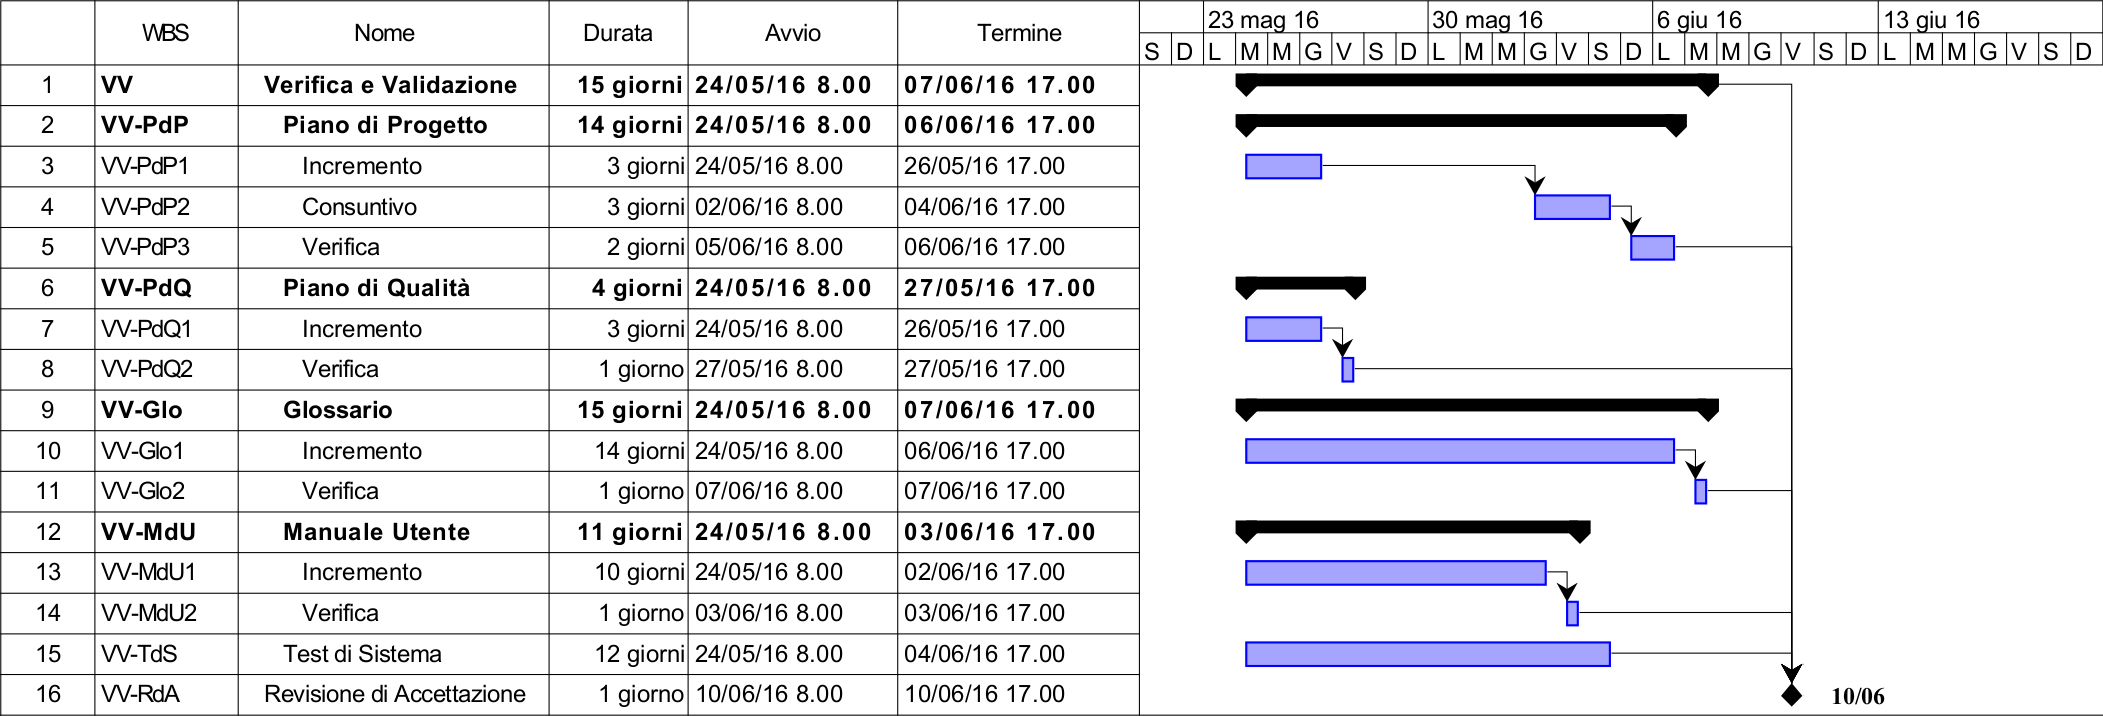
\includegraphics[keepaspectratio = true, width=16cm]{immagini/PdP_VerificaEValidazioneGantt.png}
\end{center}
\begin{figure}[h]
	\caption{\textit{Diagramma di Gantt\ped{G}} relativo al periodo di \VV.}\label{etichetta}
\end{figure}
\section{Calendario delle attività}
In questa sezione vengono presentati i quadri riassuntivi ed i grafici dell'impegno dei ruoli nei diversi periodi. infine, vengono mostrate le incidenze dei vari ruoli nell'intero progetto\ped{G}.

\subsection{Analisi dei Requisiti}
Le ore impiegate in questo periodo sono 210 e vengono ripartite in:
\begin{table}[H]
	\begin{center}
		\begin{tabular}{|c|c|}
			\hline
			\textbf{Ruolo}	& \textbf{Ore} \\
			\hline
			Responsabile	&	43	\\
			\hline
			Amministratore	&	18	\\
			\hline
			Analista		&	84	\\
			\hline
			Verificatore	&	65	\\
			\hline
		\end{tabular}
	\end{center}
	\caption{Ore a ruolo, Analisi dei Requisiti}
\end{table}

\begin{figure}[H]
	\centering
	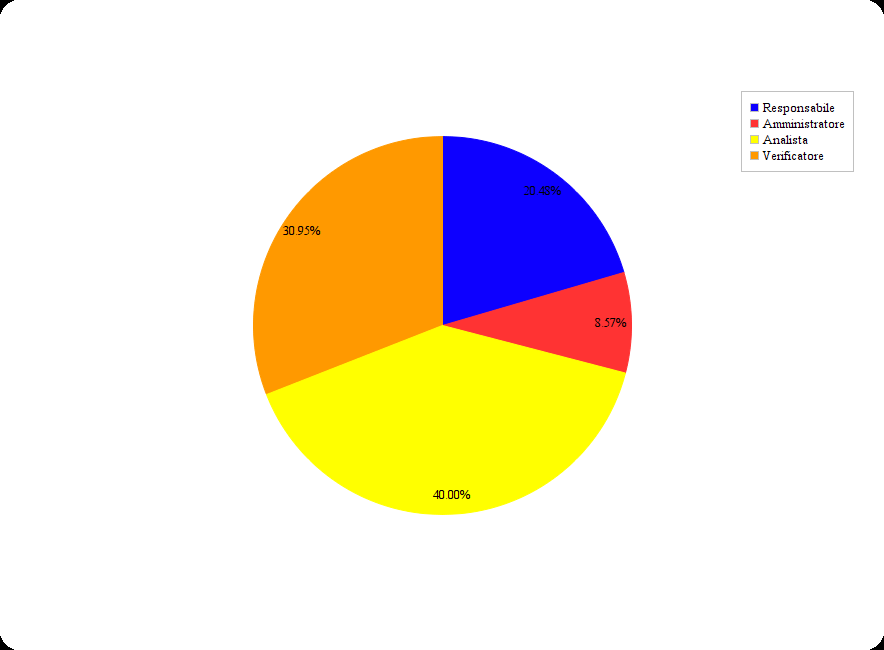
\includegraphics[scale=0.3]{immagini/Grafi/OreRuoloRR}
	\caption{Incidenza ore per ruolo, Analisi dei Requisiti}
\end{figure}

\subsection{Progettazione Architetturale}
Le ore totali impiegate in questo periodo sono 225 e vengono ripartite in:
\begin{table}[H]
	\begin{center}
		\begin{tabular}{|c|c|}
			\hline
			\textbf{Ruolo}	& \textbf{Ore} \\
			\hline
			Responsabile	&	6	\\
			\hline
			Amministratore	&	8	\\
			\hline
			Progettista		&	141	\\
			\hline
			Verificatore	&	70	\\
			\hline
		\end{tabular}
	\end{center}
	\caption{Ore a ruolo, Progettazione Architetturale}
\end{table}

\begin{figure}[H]
	\centering
	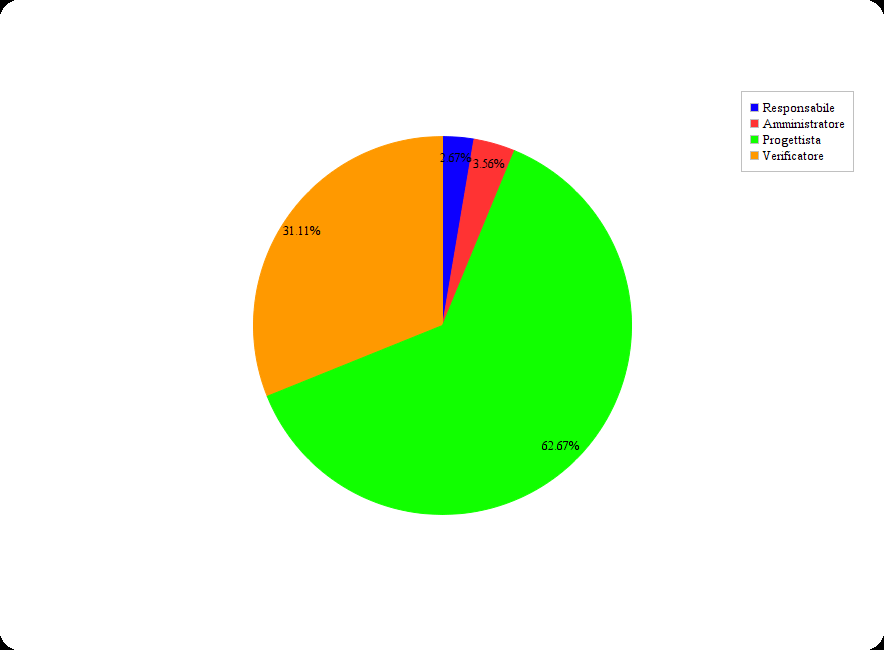
\includegraphics[scale=0.3]{immagini/Grafi/OreRuoloPA}
	\caption{Incidenza ore per ruolo, Progettazione Architetturale}
\end{figure}


\subsection{Progettazione di Dettaglio}
Le ore impiegate in questo periodo sono 140 e vengono ripartite in:
\begin{table}[H]
	\begin{center}
		\begin{tabular}{|c|c|}
			\hline
			\textbf{Ruolo}	& \textbf{Ore} \\
			\hline
			Responsabile	&	7	\\
			\hline
			Amministratore	&	5	\\
			\hline
			Progettista		&	86	\\
			\hline
			Verificatore	&	42	\\
			\hline
		\end{tabular}
	\end{center}
	\caption{Ore a ruolo, Progettazione di Dettaglio}
\end{table}

\begin{figure}[H]
	\centering
	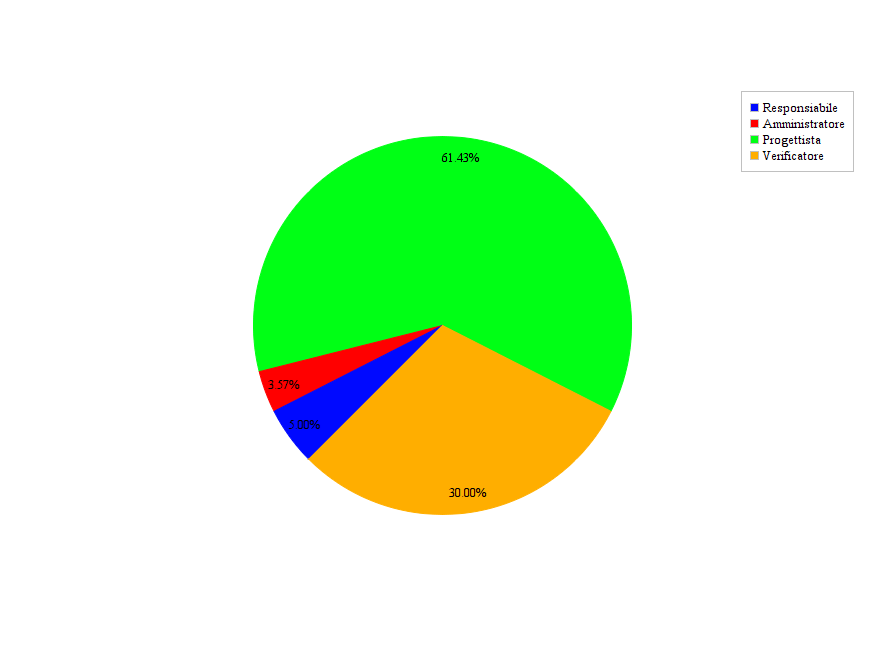
\includegraphics[scale=0.3]{immagini/Grafi/OreRuoloPD}
	\caption{Incidenza ore per ruolo, Progettazione in Dettaglio}
\end{figure}

\subsection{Codifica}
Le ore impiegate in questo periodo sono 248 e vengono ripartite in:
\begin{table}[H]
	\begin{center}
		\begin{tabular}{|c|c|}
			\hline
			\textbf{Ruolo}	& \textbf{Ore} \\
			\hline
			Responsabile	&	11	\\
			\hline
			Amministratore	&	4	\\
			\hline
			Progettista		&	25	\\
			\hline
			Programmatore	&	133	\\
			\hline
			Verificatore	&	75	\\
			\hline
		\end{tabular}
	\end{center}
	\caption{Ore a ruolo, Codifica}
\end{table}

\begin{figure}[H]
	\centering
	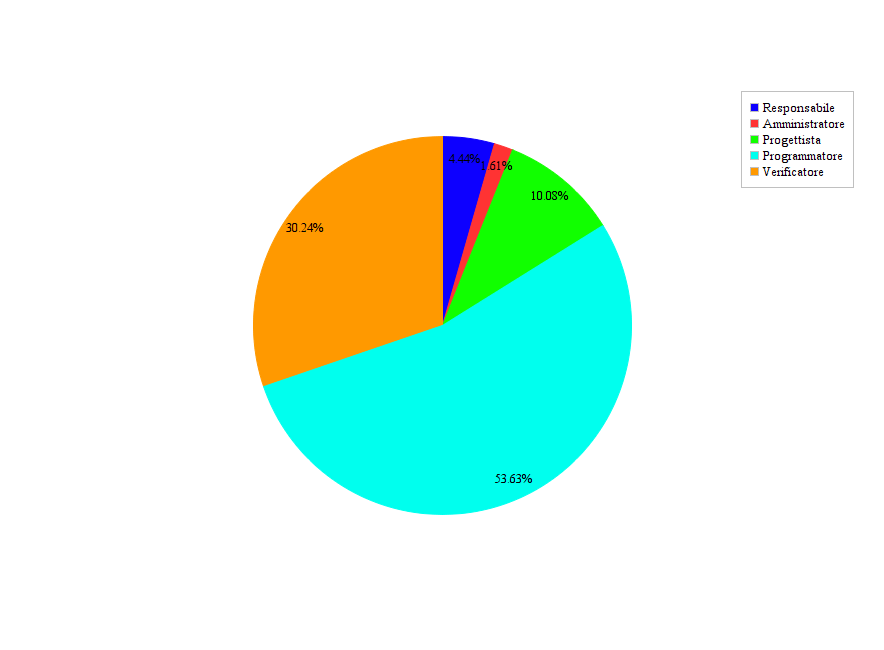
\includegraphics[scale=0.3]{immagini/Grafi/OreRuoloCod}
	\caption{Incidenza ore per ruolo, Codifica}
\end{figure}

\subsection{Verifica e Validazione}
Le ore totali in questo periodo sono 122 e vengono ripartite in:
\begin{table}[H]
	\begin{center}
		\begin{tabular}{|c|c|}
			\hline
			\textbf{Ruolo}	& \textbf{Ore} \\
			\hline
			Responsabile	&	9	\\
			\hline
			Progettista		&	20	\\
			\hline
			Verificatore	&	93	\\
			\hline
		\end{tabular}
	\end{center}
	\caption{Ore a ruolo, Verifica e Validazione}
\end{table}

\begin{figure}[H]
	\centering
	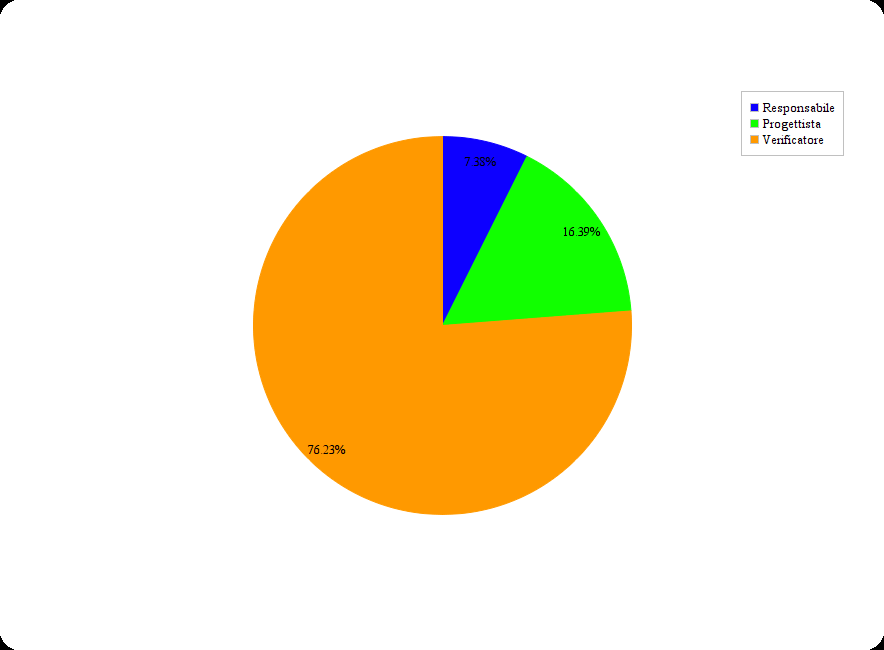
\includegraphics[scale=0.3]{immagini/Grafi/OreRuoloVerifica}
	\caption{Incidenza ore per ruolo, Verifica e Validazione}
\end{figure}

\subsection{Quadro riassuntivo}
Le ore totali del progetto\ped{G} sono 945, di cui 735 remunerabili, così ripartite:
\begin{table}[H]
	\begin{center}
		\begin{tabular}{|c|c|c|}
			\hline
			\textbf{Ruolo}	& \textbf{Ore totali} & \textbf{Ore remunerabili} \\
			\hline
			Responsabile	&	76	&	33	\\
			\hline
			Amministratore	&	35	&	17	\\
			\hline
			Analista		&	84	&	0	\\
			\hline
			Progettista		&	272	&	272	\\
			\hline
			Programmatore	&	133	&	133	\\
			\hline
			Verificatore	&	345	&	280	\\
			\hline
		\end{tabular}
	\end{center}
	\caption{Ore a ruolo, Quadro riassuntivo}
\end{table}

\begin{figure}[H]
	\centering
	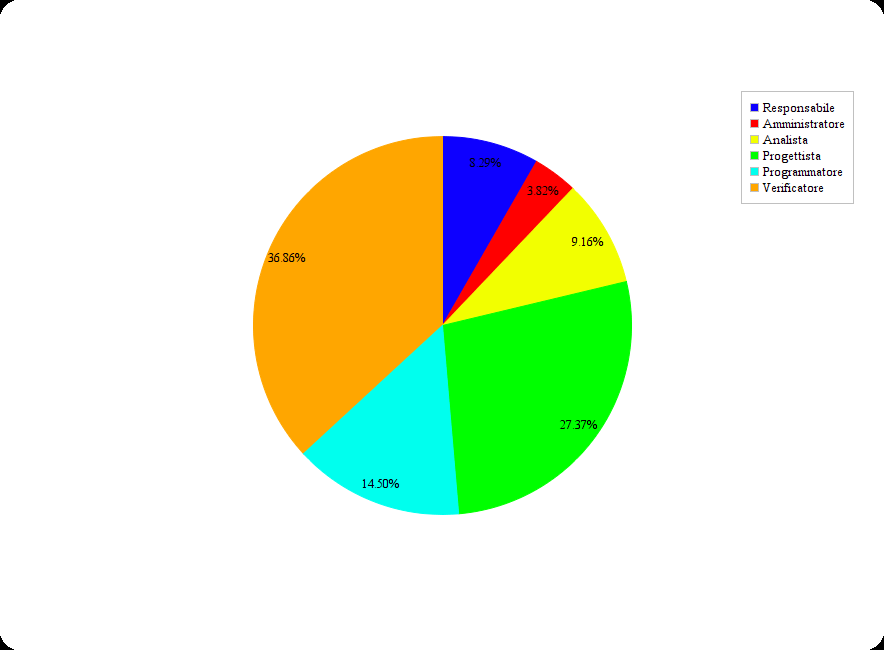
\includegraphics[scale=0.3]{immagini/Grafi/OreRuoloOreTotali}
	\caption{Incidenza ore per ruolo, Ore Totali}
\end{figure}

\begin{figure}[H]
	\centering
	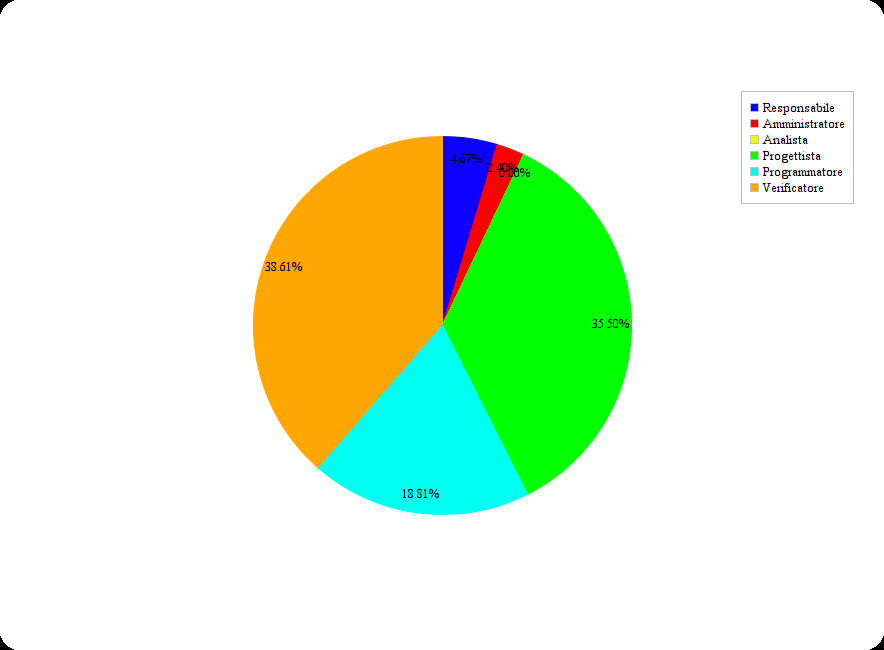
\includegraphics[scale=0.3]{immagini/Grafi/OreRuoloRendicontabili}
	\caption{Incidenza ore per ruolo, Ore Rendicontate}
\end{figure}

\section{Suddivisione del lavoro}
I componenti del gruppo dovranno rivestire ciascuno, almeno una volta, tutti i ruoli specificati nell'\textit{Organigramma\ped{G}}.
Durante le varie fasi ogni componente può ricoprire più ruoli, anche contemporaneamente, purchè non si presentino dei conflitti di interesse tra le attività svolte. Ad esempio un componente non può essere \textit{\Ver} di se stesso.
\subsection{Analisi dei Requisiti}
Nell'attività di \textit{\AdR} ciascun componente dovrà rivestire i seguenti ruoli:
\begin{table}[H]
	\begin{center}
		\begin{tabular}{|c|c|c|c|c|c|c|c|}
			\hline
			\textbf{Nominativo} & \multicolumn{6}{c|}{\textbf{Ore per ruolo}} & \textbf{Ore totali} \\
			& \textbf{Re} & \textbf{Am} & \textbf{An} & \textbf{Pj} & \textbf{Pr} & \textbf{Ve} & \\
			\hline
			\FB	&		&	4	&	23	&		&		&		&	27	\\
			\hline
			\AF		&		&	6	&	21	&	 	&		&		& 	27	\\
			\hline
			\GN		&	20	&		&	9	&		&		&		&	29	\\
			\hline						
			\GR	&	20	&	 	&	8 	&		&	 	& 		&	28	\\
			\hline
			\SM 		&		&	3	&	5	&		&		& 	20	&	28	\\
			\hline
			\MP		& 		&		&	7	&		&		&	20	&	27	\\
			\hline						
			\MV 		&		&	4	&	5	&		&		&	20	& 	29	\\
			\hline
		\end{tabular}
	\end{center}
	\caption{Ore per componente, \AdR}
\end{table}

\begin{figure}[H]
	\centering
	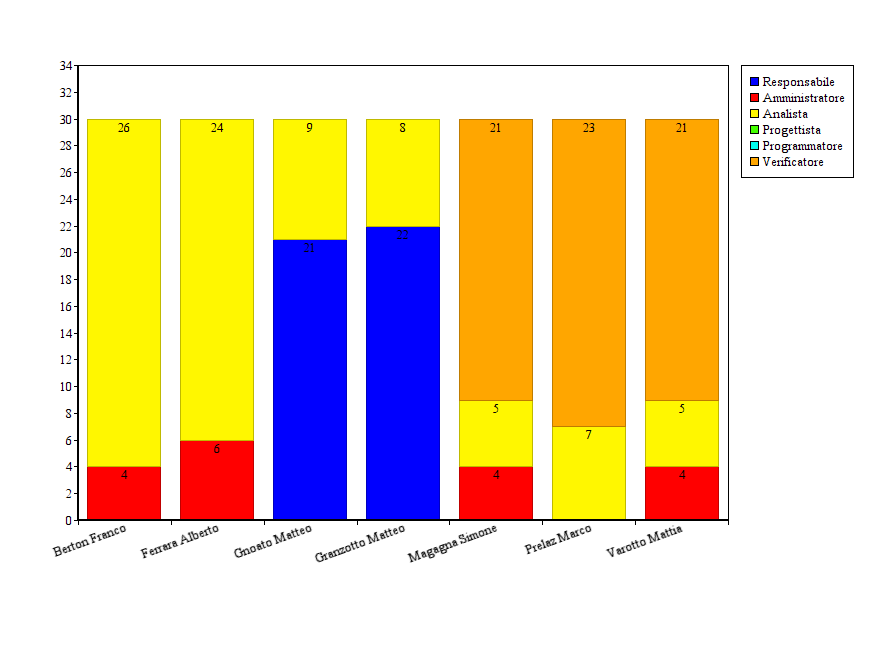
\includegraphics[scale=0.4]{immagini/Grafi/GrafoAR}
	\caption{Incidenza ore per ruolo, Analisi dei Requisiti}
\end{figure}

\subsection{Analisi dei Requisiti in Dettaglio}
Nell'attività di \textit{\AD} ciascun componente dovrà rivestire i seguenti ruoli:

\begin{table}[H]
	\begin{center}
		\begin{tabular}{|c|c|c|c|c|c|c|c|}
			\hline
			\textbf{Nominativo} & \multicolumn{6}{c|}{\textbf{Ore per ruolo}} & \textbf{Ore totali} \\
			& \textbf{Re} & \textbf{Am} & \textbf{An} & \textbf{Pj} & \textbf{Pr} & \textbf{Ve} & \\
			\hline
			\FB	&		&		&	3	&		&		&		&	3	\\
			\hline
			\AF		&		&		&	3	&	 	&		&		& 	3	\\
			\hline
			\GN		&	1	&		&		&		&		&		&	1	\\
			\hline						
			\GR	&	2	&	 	&	 	&		&	 	& 		&	2	\\
			\hline
			\SM 		&		&	1	&		&		&		& 	1	&	2	\\
			\hline
			\MP		& 		&		&		&		&		&	3	&	3	\\
			\hline						
			\MV 		&		&		&		&		&		&	1	& 	1	\\
			\hline
		\end{tabular}
	\end{center}
	\caption{Ore per componente, \AD}
\end{table}

\begin{figure}[H]
	\centering
	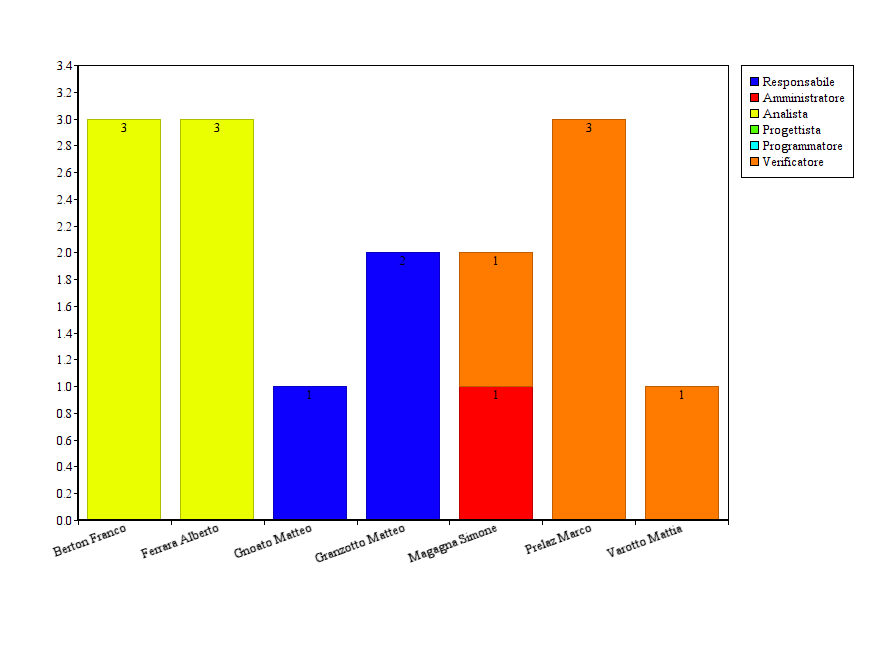
\includegraphics[scale=0.4]{immagini/Grafi/GrafoARD}
	\caption{Incidenza ore per ruolo, \AD}
\end{figure}

\subsection{Progettazione Architetturale}
Nel periodo di Progettazione Architetturale ciascun componente del gruppo dovrà rivestire i seguenti ruoli:
\begin{table}[H]
	\begin{center}
		\begin{tabular}{|c|c|c|c|c|c|c|c|}
			\hline
			\textbf{Nominativo} & \multicolumn{6}{c|}{\textbf{Ore per ruolo}} & \textbf{Ore totali} \\
			& \textbf{Re} & \textbf{Am} & \textbf{An} & \textbf{Pj} & \textbf{Pr} & \textbf{Ve} & \\
			\hline
			\FB		&		&		&		&	10	&		&	23	&	33	\\
			\hline
			\AF	&		&		&		&	9 	&		&	23	& 	32	\\
			\hline
			\GN		&		&		&		&	8	&		&	24	&	32	\\
			\hline									
			\GR	&		&	 4	&  		&	28	&	 	& 		&	32	\\
			\hline
			\SM 		&	3	&		&		&	29	&		& 		&	32	\\
			\hline
			\MP 		& 		&	4	&		&	28	&		&		&	32	\\
			\hline						
			\MV 		&	3	&		&		&	29	&		&		& 	32	\\
			\hline
		\end{tabular}
	\end{center}
	\caption{Ore per componente, Progettazione Architetturale}
\end{table}

\begin{figure}[H]
	\centering
	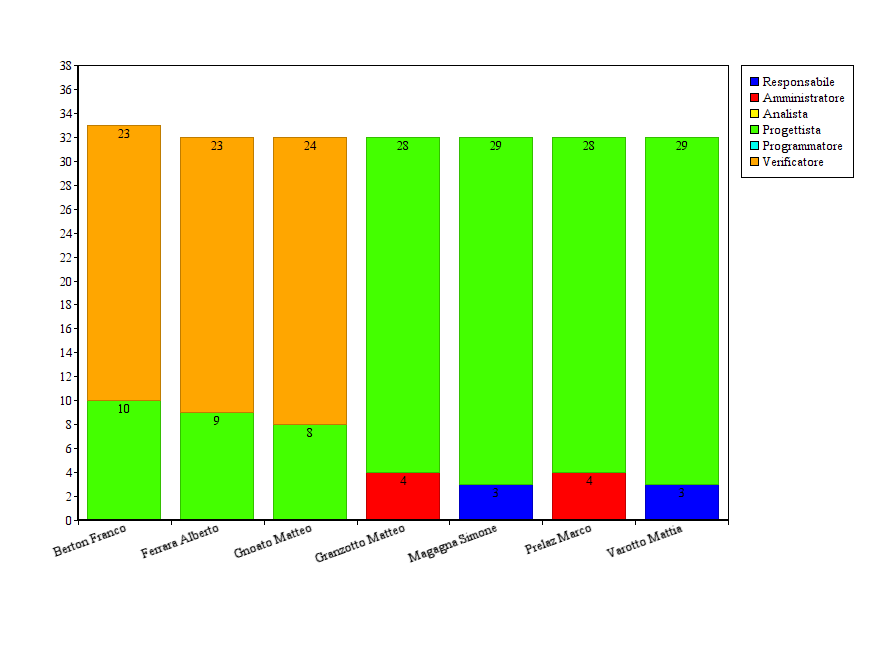
\includegraphics[scale=0.4]{immagini/Grafi/GrafoPA}
	\caption{Incidenza ore per ruolo, Progettazione Architetturale}
\end{figure}

\subsection{Progettazione di Dettaglio}
Nel periodo di Progettazione di Dettaglio ciascun componente del gruppo dovrà rivestire i seguenti ruoli:
\begin{table}[H]
	\begin{center}
		\begin{tabular}{|c|c|c|c|c|c|c|c|}
			\hline
			\textbf{Nominativo} & \multicolumn{6}{c|}{\textbf{Ore per ruolo}} & \textbf{Ore totali} \\
			& \textbf{Re} & \textbf{Am} & \textbf{An} & \textbf{Pj} & \textbf{Pr} & \textbf{Ve} & \\
			\hline
			\FB		&	3	&		&		&	17	&		&		&	20	\\ 
			\hline
			\AF		&	4	&		&		&	16	&		&		& 	20	\\ 
			\hline
			\GN		&		&	2	&		&	18	&		&		&	20	\\ 
			\hline									
			\GR	&		&	 	&		&	6	&	 	& 	14	&	20	\\
			\hline
			\SM 		&		&	3	&		&	17	&		& 		&	20	\\ 
			\hline
			\MP 		& 		&		&		&	6	&		&	14	&	20	\\ 
			\hline
			\MV 		&		&		&		&	6	&		&	14	& 	20	\\ 
			\hline
		\end{tabular}
	\end{center}
	\caption{Ore per componente,Progettazione di Dettaglio}
\end{table}

\begin{figure}[H]
	\centering
	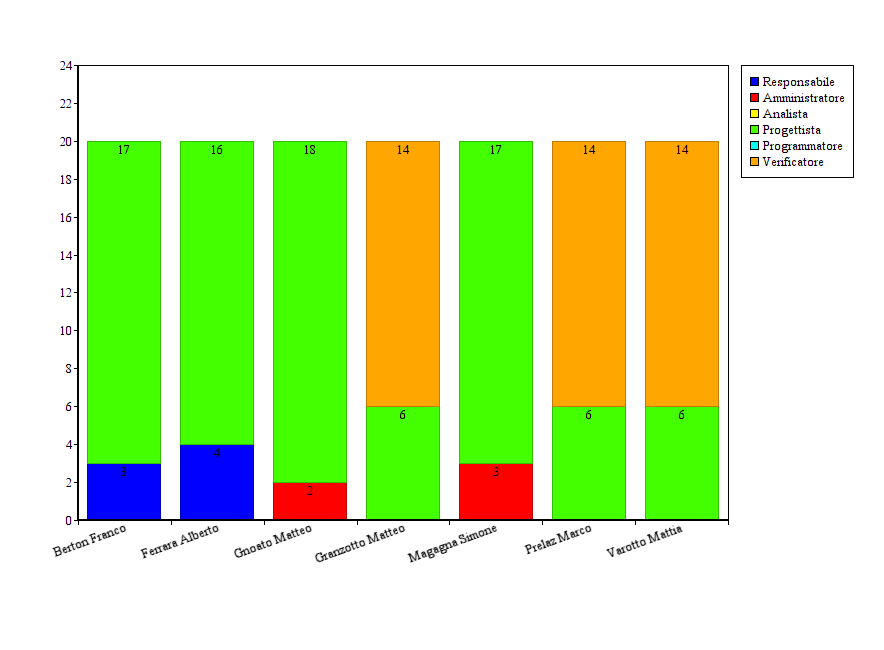
\includegraphics[scale=0.4]{immagini/Grafi/GrafoPD}
	\caption{Incidenza ore per ruolo, Progettazione di Dettaglio}
\end{figure}

\subsection{Codifica}
Nel periodo di Codifica ciascun componente del gruppo dovrà rivestire i seguenti ruoli:
\begin{table}[H]
	\begin{center}
		\begin{tabular}{|c|c|c|c|c|c|c|c|}
			\hline
			\textbf{Nominativo} & \multicolumn{6}{c|}{\textbf{Ore per ruolo}} & \textbf{Ore totali} \\
			& \textbf{Re} & \textbf{Am} & \textbf{An} & \textbf{Pj} & \textbf{Pr} & \textbf{Ve} & \\
			\hline
			\FB		&		&		&		&		&	35	&		&	35	\\
			\hline	
			\AF		&		&		&		&	 5	&	31	&		& 	36	\\
			\hline		
			\GN		&		&	4	&		&		&	7	&	25	&	36	\\
			\hline						
			\GR	&	5	&	 	&		&	5	&	25 	& 		&	35	\\
			\hline
			\SM 		&		&		&		&	5	&	5	& 	25	&	35	\\
			\hline
			\MP 		& 	6	&		&		&	5	&	24	&		&	35	\\
			\hline
			\MV 		&		&		&		&	5	&	6	&	25	& 	36	\\
			\hline			
		\end{tabular}
	\end{center}
	\caption{Ore per componente, Analisi dei Requisiti}
\end{table}

\begin{figure}[H]
	\centering
	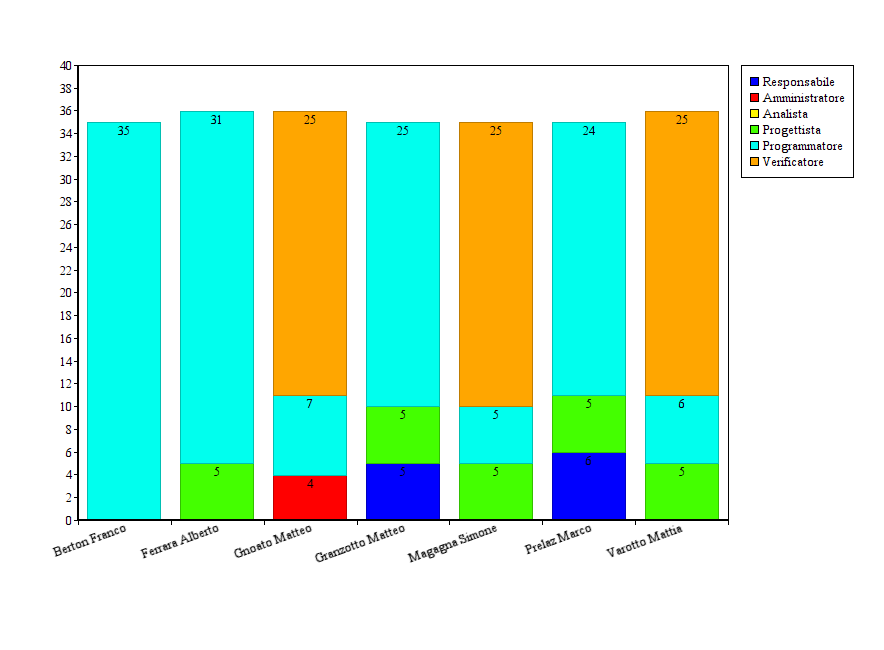
\includegraphics[scale=0.4]{immagini/Grafi/GrafoCod}
	\caption{Incidenza ore per ruolo, Codifica}
\end{figure}

\subsection{Verifica e Validazione}
Nel periodo di Verifica e Validazione ciascun componente del gruppo dovrà rivestire i seguenti ruoli:
\begin{table}[H]
	\begin{center}
		\begin{tabular}{|c|c|c|c|c|c|c|c|}
			\hline
			\textbf{Nominativo} & \multicolumn{6}{c|}{\textbf{Ore per ruolo}} & \textbf{Ore totali} \\
			& \textbf{Re} & \textbf{Am} & \textbf{An} & \textbf{Pj} & \textbf{Pr} & \textbf{Ve} & \\
			\hline
			\FB		&		&		&		&	6	&		&	11	&	17	\\
			\hline
			\AF		&		&		&		&	 6	&		&	11	& 	17	\\
			\hline	
			\GN		&		&		&		&	8	&		&	9	&	17	\\
			\hline								
			\GR	&		&	 	&		&		&	 	& 	18	&	18	\\
			\hline
			\SM 		&	9	&		&		&		&		& 	9	&	18	\\
			\hline	
			\MP 		& 		&		&		&		&		&	18	&	17	\\
			\hline					
			\MV 		&		&		&		&		&		&	17	& 	17	\\
			\hline
		\end{tabular}
	\end{center}
	\caption{Ore per componente, Verifica e Validazione}
\end{table}

\begin{figure}[H]
	\centering
	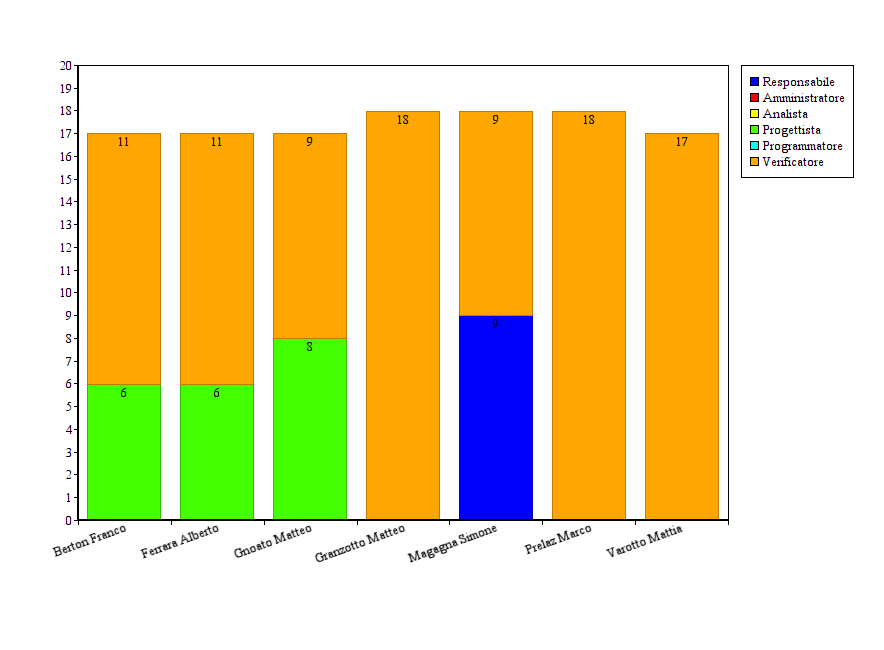
\includegraphics[scale=0.4]{immagini/Grafi/GrafoVV}
	\caption{Incidenza ore per ruolo, Verifica e Validazione}
\end{figure}

\subsection{Totali}
La tabella seguente illustra le ore totali che ogni componente dedicherà per il progetto, mettendo in evidenza anche quelle che verranno poi rendicontate.
\begin{table}[H]
	\begin{center}
		\begin{tabular}{|c|c|c|c|c|c|c|c|c|}
			\hline
			\multirow{2}{*}{\textbf{Nominativo}} & & \multicolumn{6}{c|}{\textbf{Ore per ruolo}} & \multirow{2}{*}{\textbf{Ore totali}} \\
			& & \textbf{Re} & \textbf{Am} & \textbf{An} & \textbf{Pj} & \textbf{Pr} & \textbf{Ve} & \\
			\hline
			\hline
			\multirow{2}{*}{\FB}		&	Rendicontate	&	3	&	0	&	0	&	33	&	35	& 34 	&	105	\\
			\cline{2-9}
			&	Totali			&	3	&	4	&	26	&	33	&	35	& 	34	&	135	\\
			\hline	
			\hline
			\multirow{2}{*}{\AF}	&	Rendicontate	&	4	&	0	&	0	&	35	&	31	&  34	&	105	\\
			\cline{2-9}
			&	Totali			&	4	&	6	&	24	&	35	&	31	& 	34	&	135	\\
			\hline
			\hline
			\multirow{2}{*}{\GN}	&	Rendicontate	&	0	&	6	&	0	&	34	&	7	&	58	&	105	\\
			\cline{2-9}
			&	Totali			&	21	&	6	&	9	&	34	&	7	&	58	&	135	\\
			\hline
			\hline					
			\multirow{2}{*}{\GR}	&	Rendicontate	&	5	&	4	&	0	&	39	&	25	&	32	&	105	\\
			\cline{2-9}
			&	Totali			&	27	&	4	&	8	&	39	&	25	&	32	&	135	\\
			\hline
			\hline
			\multirow{2}{*}{\SM}		&	Rendicontate	&	12	&	3	&	0	&	51	&	5	& 	34	&	105	\\
			\cline{2-9}
			&	Totali			&	12	&	7	&	5	&	51	&	5	& 	55	&	135	\\
			\hline			
			\hline
			\multirow{2}{*}{\MP}	&	Rendicontate	&	6	&	4	&	0	&	39	&	24	& 	32	&	105	\\
			\cline{2-9}
			&	Totali			&	6	&	4	&	7	&	39	&	24	& 	55	&	135	\\
			\hline
			\hline			
			\multirow{2}{*}{\MV}	&	Rendicontate	&	3	&	0	&	0	&	40	&	6	& 	56	&	105	\\
			\cline{2-9}
			&	Totali			&	3	&	4	&	5	&	40	&	6	& 	77	&	135	\\
			\hline
		\end{tabular}
	\end{center}
	\caption{Ore per componente per ruolo, rendicontate e totali}
\end{table}

\section{Prospetto economico}
\subsection{Analisi dei Requisiti}
\subsection{Progettazione e Codifica}
\subsubsection{Progettazione Architetturale}
\subsubsection{Progettazione di Dettaglio}
\subsubsection{Codifica}
\subsection{Verifica e Validazione}
\subsection{Prospetto finale}
\subsection{Conclusioni}
\newpage
\section{Meccanismi di controllo e di rendicontazione}
	\subsection{Meccanismi di controllo} Sono stati adottati dei meccanismi, nell'ambiente creato, per:
	\begin{itemize}
		\item Controllare l'andamento delle attività;
		\item Permettere un aggiornamento facilitato della pianificazione;
		\item Rendicontare le ore di lavoro spese nelle varie attività.
	\end{itemize}
	\subsection{Controllo ritardi di attività}  Per mantenere il controllo sull'andamento generale si è scelto di adottare dei metodi grafici.
		\subsubsection{Dettaglio attività} Il sistema di ticketing adottato permette di visualizzare in modo dinamico il \textit{diagramma di  Gantt\ped{G}} delle attività. Viene visualizzato:
		\begin{itemize}
			\item La percentuale di completamento di ognuna di esse;
			\item Le attività in ritardo;
			\item Le attività concluse.
		\end{itemize}
		\begin{center}
			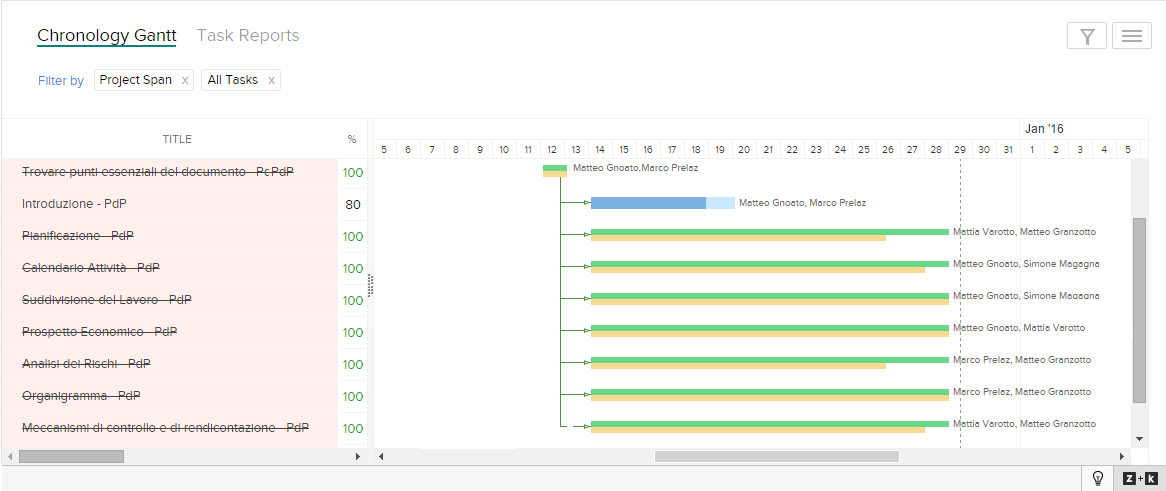
\includegraphics[keepaspectratio = true, width=16cm]{immagini/PdP_ZohoGantt.png}
		\end{center}
		\begin{figure}[h]
			\caption{\textit{Diagramma di Gantt\ped{G}} prodotto dal sistema di ticketing adottato.}\label{etichetta}
		\end{figure}
		\subsubsection{Fasi processi}
		Combinando i dati del sistema di ticketing in un grafico ad area in pila per visualizzare il numero di ticket aperti in un particolare stato del \textit{ciclo di Deming\ped{G}}, è immediato visualizzare in quali stati si trovino le attività.
		\subsubsection{Controllo date} Per ottimizzare la pianificazione e tenerla in costante aggiornamento si utilizzano dei calendari a disposizione del gruppo.
		\subsubsection{Calendario attività}
		Il sistema di ticketing adottato genera automaticamente un calendario in cui vengono indicate inizio e fine delle varie attività.
		\subsubsection{Calendario risorse} Il calendario a disposizione del gruppo utilizzato per gestire il personale in base agli impegni dei vari componenti.
		\subsubsection{Controllo metriche di progetto} L'introduzione delle metriche consente di quantificare nel modo più obiettivo possibile le performance del gruppo nello svolgimento del progetto attraverso la misurazione dell'insieme di indicatori che ne fanno parte. Tipicamente uno degli usi più importanti delle metriche è quello di misurare l'avanzamento del progetto a fronte del piano. Il loro utilizzo consente di: 
		\begin{itemize}
			\item Identificare i problemi di costo/schedulazione prima che diventino criticità;
			\item Aiutare il \textit{team\ped{G}} a focalizzarsi sul completamento delle proprie attività.
		\end{itemize}
		In particolare le metriche \textit{Budget Variance\ped{G}}(BV) e \textit{Schedule Variance\ped{G}}(SV) permettono rispettivamente di:
		\begin{itemize}
			\item Indicare se si è speso di più o di meno rispetto a quanto previsto;
			\item Indicare se si è in linea, in anticipo o in ritardo rispetto alla schedulazione delle	attività di progetto pianificate nella \textit{baseline\ped{G}}. 
		\end{itemize}
		I valori aggiornati di tali metriche sono riportati nel \textit{\PdQ}.
	\subsection{Meccanismi di rendicontazione} Il sistema di ticketing adottato mette a disposizione la rendicontazione delle ore di lavoro. Tale sistema permette di visualizzare le ore di lavoro in base all'attività svolta.
\appendix
\section{Analisi dei rischi}
\subsection{}
\newpage
\section{Organigramma}
\subsection{Redazione}
\begin{table}[htbp]
	\begin{center}
		\setlength{\extrarowheight}{\jot}
		\begin{tabular}{|c|c|p{6cm}|}
			\hline
			\textbf{Nominativo} & \textbf{Data di redazione} & \textbf{Firma} \\[1ex]
			\hline
			\GR & 2016-01-07 & \myincludegraphics{immagini/Firme/MGR.png} \\[1ex]
			\hline
		\end{tabular}
	\end{center}
	\caption{Redazione}
\end{table}

\subsection{Approvazione}
\begin{table}[htbp]
	\begin{center}
		\setlength{\extrarowheight}{\jot}
		\begin{tabular}{|c|c|p{5cm}|}
			\hline
			\textbf{Nominativo}     & \textbf{Data di approvazione} & \textbf{Firma}  \\[1ex]
			\hline
			\GR		& 2016-01-07					& \myincludegraphics{immagini/Firme/MGR.png}			\\[1ex]
			\hline
			\TV	&								&			\\[1ex]
			\hline
		\end{tabular}
	\end{center}
	\caption{Approvazione}
\end{table}

\subsection{Accettazione dei componenti}
\begin{table}[htbp]
	\begin{center}
		\setlength{\extrarowheight}{\jot}
		\begin{tabular}{|c|c|p{6cm}|}
			\hline
			\textbf{Nominativo} & \textbf{Data di accettazione} & \textbf{Firma} \\[1ex]
			\hline
			\GR	&	2016-01-07	& \myincludegraphics{immagini/Firme/MGR.png}	\\[1ex]
			\hline
			\GN		&	2016-01-07	& \myincludegraphics{immagini/Firme/MGN.png}		\\[1ex]
			\hline
			\AF		&	2016-01-07	& \myincludegraphics{immagini/Firme/AF.png}		\\[1ex]
			\hline
			\FB		&	2016-01-07	& \myincludegraphics{immagini/Firme/FB.png}		\\[1ex]
			\hline
			\MP		&	2016-01-07	& \myincludegraphics{immagini/Firme/MP.png}		\\[1ex]
			\hline
			\SM		&	2016-01-07	& \myincludegraphics{immagini/Firme/SM.png}		\\[1ex]
			\hline
			\MV		&	2016-01-07	& \myincludegraphics{immagini/Firme/MV.png}		\\[1ex]
			\hline
		\end{tabular}
	\end{center}
	\caption{Accettazione}
\end{table}

\subsection{Componenti}
\begin{table}[H]
	\begin{center}
		\setlength{\extrarowheight}{\jot}
		\begin{tabular}{|c|c|p{5cm}|p{4.3cm}|}
			\hline
			\textbf{Nominativo} & \textbf{Matricola} & \raggedright \textbf{Indirizzo di posta elettronica} & \textbf{Ruoli} \\[1ex]
			\hline
	 		\GR	& 1051540	& \href{mailto:granzotto.matteo@gmail.com}{granzotto.matteo@gmail.com} 	& \Res, \Ana 	\\[1ex]
			\hline
			\GN		& 1051873	& \href{mailto:gnoatomatteo@gmail.com}{gnoatomatteo@gmail.com} 			& \Res, \Ana 	\\[1ex]
			\hline
			\AF		& 1049378	& \href{mailto:albertoferrara92@gmail.com}{albertoferrara92@gmail.com} 	& \Amm, \Ana 	\\[1ex]
			\hline
			\FB 		& 1052574	& \href{mailto:franco.berton93@gmail.com}{franco.berton93@gmail.com} 	& \Amm, \Ana	\\[1ex]
			\hline
			\MP		& 1047343	& \href{mailto:marcomak91@hotmail.it}{marcomak91@hotmail.it} 			& \Ver, \Ana	\\[1ex]
			\hline
			\SM		& 1009467	& \href{mailto:simone.magagna91@gmail.com}{simone.magagna91@gmail.com} 	& \Ver, \Ana, \Amm 	\\[1ex]
			\hline
			\MV		& 1051619	& \href{mailto:varots93@hotmail.it}{varots93@hotmail.it} & \Ver, \Ana, \Amm \\[1ex]
			\hline	
		\end{tabular}
	\end{center}
	\caption{Componenti}
\end{table}



\end{document}